%%%%%%%%%%%%%%%%%%%%%%%%%%%%%%%%%%%%%%%%%%%%%%%%%%%%%%%%%%%%%%%%%%%%%%%%%%%%%%%%%%%%%%%%%%%%%
%%									Chapitre Contribution											%
%%%%%%%%%%%%%%%%%%%%%%%%%%%%%%%%%%%%%%%%%%%%%%%%%%%%%%%%%%%%%%%%%%%%%%%%%%%%%%%%%%%%%%%%%%%%%
\chapter{Algorithme de distribution d’espace d’états basée sur le comportement des systèmes}
%	\citationChap{
%	...
%	}{...}

%%%%%%%%%%%%%%%%%%%%%%%%%%%%%%%%%%%%%%%%%%%%%%%%%%%%%%%%%%%%%%%%%%%%%%%%%%%%%%%%%%%%%%%%%%%%%
 \section{Introduction}
Dans les travaux \citep{Saidouni2012}, \citep{TabibSaidouni2016}, \citep{BENSETIRA2017}, nous avons constaté que les méthodes de génération des espaces d’états pour le model checking consiste  qu’un grand espace d'états non structuré soit divisé en parties de tailles équilibrées, de telle sorte que peu de transitions lient les différentes  parties, car chaque transition externe peut entraîner une surcharge de communication.

Après une étude des espaces d'états générés, nous avons constaté que la diminution de transitions liant les différentes parties peut entraîner un mauvais équilibrage de charge entre les machines du réseau. Outre l’équilibrage de charge, il peut entraîner une mauvaise qualité de distribution de l'espace d'états car lorsqu'une formule du model checking n'est pas vérifiée sur un état la diminution de transitions externes n'empêche pas une surcharge de communication. La qualité de distribution est estimée en fonction de la quantité de communication requise pour l’exécution des tâches distribuées \citep{EzekielLuttgen2008}. Ainsi La réalisation de ces objectifs nécessiterait des informations supplémentaires sur l’espace d’états considéré et les communications engendrées. 

Ces raisons nous ont amené à proposer une nouvelle politique de redistribution qui vise à analyser le comportement d’un système donné en générant son espaces d’états et en extrayant les informations pertinentes sur les états et leurs connexions (transitions internes et externes). Ensuite, redistribuer les états pertinents selon une certaines heuristiques basé sur la théorie de jeux afin d’optimiser les performances du système. les machines sont considérées comme des joueurs, Chaque machine cherche a optimisée ces performances en définissant une bonne localité pour un état pertinent tout en optimise l’équilibre de charge et la quantité de communication entre les machines.
 
Dans ce qui suit nous présentons la nouvelle politique de redistribution de l’espace d’états basée sur le comportement du système ainsi que les résultats obtenus. 
 

\section{Politique de distribution de l’espace d’états basée sur le	comportement du système}
 
La politique proposée \emph{\BbSSD{}}, vise à optimiser la distribution de l’espace d’états ainsi le temps de vérification du model checking. Pour un système donné spécifier a partir d'un réseau de Petri, nous utilisons un algorithme de génération parallèle pour construire la structure de Kripke distribuée, en utilisant la fonction \emph{MD5} pour le partitionnement de l’espace d’états entre les machines du réseau. Après cela, lors de l'exécution du model checking, chaque machine analyse son fragment (structure de Kripke partiale) et élabore certaines statistiques sur les états par rapport a la vérification. Les statistiques  générer sur chaque état mesure la dépendance de l'état par rapport aux états de la machine local ou aux états des machines distantes. Une fois le processus de vérification du model checking est terminé, Le protocole de redistribution peut être lancer afin de calculer pour chaque état \emph{Externe} et \emph{soliciter} sur lesquels la formule n'est pas vérifiée l'ensembles des états à déplacer et à dupliquer. Après le calcul des ensembles on décide, sur la base de l'écart minimum et maximum des états a stocké sur la machine, si l'ensemble peut être déplacer ou rester dans une machine afin de minimiser la quantité de communication entre les machines avec une bonne distribution, ainsi les transitions externes peut être réduit.
L’algorithme général est l'Algorithme \ref{bbssd} :\\
\begin{algorithm}[H]\label{bbssd}
	\SetAlgoLined
	\SetKwIF{If}{ElseIf}{Else}{if}{then}{else if}{else}{endif}
	 Générer la structure de Kripke distribuée à partir de la spécification d'un réseau de Petri\;
	 Exécution du model checking et élaboration des statistiques sur chaque état\;
	 Redistribuer des états, en optimisant les performances du système\;	  
	\caption{\BbSSD{}}
\end{algorithm}

Dans les sections suivantes, nous détaillons les phases de cet algorithme.

\subsection{Génération de l’espace d’états distribuée à partir de la spécification d'un réseau de Petri}{
La spécification du réseau de Petri est faite à partir d'une machine choisie aléatoirement. Le processus de génération de l'espace d'états distribuée est fait par l’exploration de l’état initial en générant tous ses états successeurs. Par la suite, toutes les machines disponibles sur le réseau contribuent à la construction des fragments de l’espace d’états distribué. Pour chaque nouvel état généré appartenant à une machine $M_i$, tous ses états successeurs sont générés. Un état successeur peut être dans la même machine ou dans une machine distante. Chaque machine $M_i$ envoie tous ses états externes aux machines déterminées par la fonction de partition. La fonction de partition est basée sur la fonction de hachage cryptographique \emph{MD5} qui renvoie un index $j\;(j \in 0, N-1)$. La fonction de hachage adoptée réalise un bon équilibrage de charge entre les $N$ machines du réseau.  La génération distribuée se termine lorsqu'il n'y a aucun états en attente d'être exploré.\\
L’algorithme de génération de l’espace d’états distribuée est l'Algorithme \ref{gendistribuer} :\\
\SetKwFunction{printlcs}{}
\begin{algorithm}
	\SetAlgoLined
	\SetKwIF{If}{ElseIf}{Else}{if}{then}{else if}{else}{endif}
	\SetAlgoLined	
	\SetKwInOut{Mi}{$M_i$}
	\SetKwInOut{Mj}{$M_j$}
	\SetKwInOut{etati}{$Etat_i$}
	\SetKwInOut{ei}{$E_i$}
	\SetKwInOut{si}{$S_i$}
	\SetKwInOut{t}{$t$}
	\SetKwInOut{T}{$T$}
	\SetKwInOut{smm}{$s,m,m'$}
	\SetKwInOut{tb}{$t_b$}
	\SetKwInOut{sm}{$s.m$}
	\SetKwInOut{sprp}{$s.L$}
	\SetKwInOut{te}{$TExplore$}
	\SetKwInOut{tr}{$TR_i$}
	\SetKwInOut{Pres}{$Pres$} 
	\SetKwInOut{Post}{$Post$}
	\SetKwInOut{pps}{$Prop\_Pres$}
	\SetKwInOut{ppt}{$Prop\_Post$}
	\AlgoDontDisplayBlockMarkers\SetAlgoNoEnd\SetAlgoNoLine%
	\Mi{machine i}
	\Mj{machine j}
	\etati{\{dehors,dedans\}}
	\ei{init à $\emptyset$, pile des états non encore explorés appartenant à la machine i}
	\si{init à $\emptyset$, la liste des états déjà explorés appartenant à la machine i }
	\smm{un état}
	\sm{marquage d'un états}
	\sprp{liste des propriétés d'un états}
	\tr{la liste des relations de transitions de la machine i}
	\T{a liste de transitions}
	\tb{transition bloquant}
	\te{liste transition admissible}
	\t{une transition}
	\Pres{matrice pres du réseau de Petri}
	\Post{matrice post du réseau de Petri}
	\pps{matrice pres des propriétés}
	\ppt{matrice post des propriétés}

	 \caption{Génération Initiale Distribuée}\label{gendistribuer}
\end{algorithm}

\begin{algorithm}
	\LinesNumbered
	% This is to restore vline mode if you did not take the package as \usepackage[linesnumbered,ruled,vlined]{algorithm2e}
	\SetAlgoVlined 
	\SetKwFunction{algo}{}\SetKwFunction{proc}{proc}
	\Begin{	 
	 \SetKwProg{myalg}{Reception Etat}{}{}
	 
	 \myalg{\algo{m:etat}envoyé par $M_j$}{  
	 	$s\leftarrow findByMarquage(m,S_i)$\;	
	 	\uIf{($ s ==null$)}{
	 		$m.sub\leftarrow\{ M_j \}$\;
	 		Empiler(m,$E_i$)\;	 		
	 		\If{($Etat_i$!= dedans)}{
	 			GenerationDistribue$_i$()\;
 			}
	 	}
 		\Else{
 		   ajouter $M_i$ à la liste des machines de l'etat portant identifiant \emph{m} \;			
 		}	 		  		
	 }{} 	  	
   	\SetKwProg{myalgone}{GenerationDistribue$_i$}{}{}   
  	 \myalgone{\algo{}}{  
	  	$Etat_i\leftarrow dedans$\;	
	  	\While{($ E_i !=\emptyset$)}{
	  		$m\leftarrow depiler(E_i)$\;
	  		$TExplore \leftarrow \{t\in T\mid m.m[t>\}$\;
	  		$S_i\leftarrow S_i \cup \{m\}$\;
	  		\ForEach{($t \in TExplore$)}{
	  			$m'.m\leftarrow m.m + Post(t)-Pres(t)$\; 
	  			$m'.L\leftarrow m.L + Prop\_Post(t)-Prop\_Pres(t)$\; 
	  			$M_j \leftarrow MD5(m'.m)$\;
	  			\uIf{$M_j = =M_i$}{
	  				$s\leftarrow findByMarquage(m,S_i)$\;
	  				\If{(findByMarquage(m'.m,$S_i$)==null and findByMarquage(m'.m,$E_i$)==null)}{
	  					Empiler(m',$E_i$)\;
	  				}
  				}\Else{  				
  					Envoyer (m') à $M_j$\;
  				}
  				$TR_i\leftarrow TR_i\cup \{(m,t,m')\}$	\;
  			}	
	  			
	  		\If{(TExplore== $\emptyset$)  }{
	  		 	$TR_i\leftarrow TR_i\cup \{(m,t_b,m)\}$\;
	  		}
  		}
	  	$Etat_i\leftarrow dehors$\;
	  }{}
  }
 	 \SetKwProg{myalgone}{Initialisation}{}{ }
  	 \myalgone{\algo{}}{  
  	 $T\leftarrow init$\;
  	 $Pres\leftarrow init$\;
  	 $Post\leftarrow init$\;
  	 $Prop\_Pres\leftarrow init$\;
  	 $Prop\_Post\leftarrow init$\;
  	 $m.m\leftarrow init$\;
  	 $m.prop\leftarrow init$\;
  	 $M_i \leftarrow MD5(m.m)$\;
  	 Envoyer (m) à $M_j$\;
  
  }
	
\end{algorithm} 
}
\pagebreak
%%%%%%%%%%%%%%%%%%%%%%%%%%%%%%%%%%%%%%%%%%%%%%%%%%%%%%%%%%%%%%%%%%%%%%%%%%%%%%%%%%%%%%%%%%%%%
%%									section 1.	Principe Mod\`{e}le Checker Distribu\'{e}											%
%%%%%%%%%%%%%%%%%%%%%%%%%%%%%%%%%%%%%%%%%%%%%%%%%%%%%%%%%%%%%%%%%%%%%%%%%%%%%%%%%%%%%%%%%%%%%

\subsection{Principe du Model Checking Distribu\'{e}}
 
Le model checking adopté est celui qui a été  propos\'{e} par Bouneb Zine dans sa thèse \citep{depriester2011bouneb} (voir chapitre \ref{chapmc}, section \ref{mcd}), permet une vérification parallèle d’une formule $\varphi$  sur les fragments de la structure de Kripke distribuée. Du fait de la distribution, la vérification de $\varphi$ d'un certain état \emph{S} dépend de la vérité en \emph{S’} de cette formule, \emph{S’}  hébergé dans une  machine distante $M_j$. La machine $M_i$ effectue la vérification de $\varphi$ sur le fragment détenue en considérant la valeur logique de \emph{S’} indécidable  $L (\emph{S’},\varphi )=\perp$ car la formule $\varphi$ peut être vérifiée en \emph{S’}. Lorsque la machine $M_j$ termine le calcul est que la formule est vérifiée en \emph{S’}, aucune notification n'est envoyée à la machine $M_i$, la machine $M_i$ considère que la formule est vérifiée en \emph{S’}, sinon la machine $M_j$ envoi à la machine $M_i$ la valeur logique de \emph{S’} qui est $L(\emph{S’}, \varphi) =false$. Dans ce cas, $M_i$ reprend le calcul de vérification avec la prise en compte de valeur logique envoyée afin de déterminer la logique de formule sur les états prédécesseurs. Une fois la terminaison est détectée, la machine détenant l’état initial déduit la véracitée de la formule $\varphi$.

\begin{Exemple}
   Soit une structure de Kripke distribuée représentée sur la Figure \ref{skd1}, les scénarios de l'exécution du model checking de la formule \s{AG(a)} sur cette structure sont:
   \begin{itemize}
   	\item Après une première itération l'algorithme détecte sur la machine $M_1$ que la formule n’est pas vérifiée sur l’état \s{S1}, cela nécessite l'envoyer d'une notification à la machine $M_3$ qui possède un prédécesseur direct de cet état.
   	\item Après la réception d'une notification sur la machine $M_3$ et la prise en compte de la notification sur l'état \s{S1}, l'algorithme du model checking est relancé sur la machine $M_3$. Après le processus de vérification, la valeur logique de la formule sur l’état \s{S5} est $false$ grâce à la deuxième itération. Après cela, aucune notification n'a été envoyé, sur la machine $M_3$ l'algorithme déduit alors la véracitée de la formule.
   \end{itemize}    
Les résultats observés durant le processus de vérification de la formule \s{AG(a)} sont représentés dans le Tableau \ref{statistique}, les lignes représentent les données concernant un état et les colonnes les types de données construits durant le processus de vérification. Les abréviations utilisées sont:
\begin{description}[,leftmargin=2cm,labelindent=1em]
	\item[Id   :] L'identifiant de l’état;
	\item[VL   :] La valeur logique de la formule à vérifier $(true : 1 ; false : 0 ; \perp : -1)$;
	\item [Sub :] Liste des machines sollicitant l'état;
	\item[T    :] Le type d’état (I : interne ; E : externe);
	\item[Site :] La machine distante o\`{u} l'état (Externe) réside;
	\item[I    :] La liste des itérations permettant de déterminer la valeur logique de l'état.	
\end{description}
   \centering
	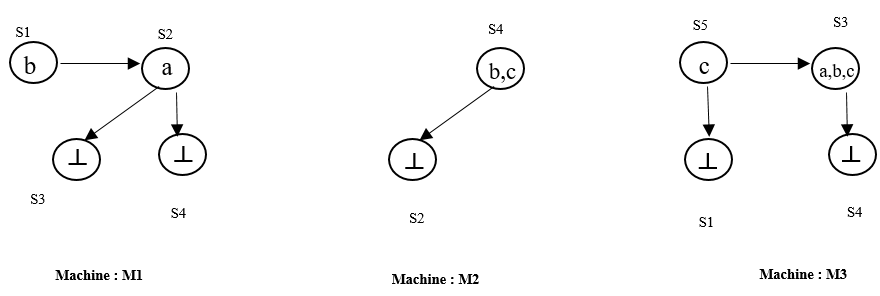
\includegraphics[height=2in]{img/skd1.png}	
	\captionof{figure}{Structure de kripke distribu\'{e}}\label{skd1}
\end{Exemple}
\begin{tableth}
	\centering
	\begin{tabular}{|c|c|c|c|c|c|c|c|c|}
		\hline
		\multicolumn{7}{|c|}{Itération 1}                                  \\ \hline
		          Machine           & Id & T & VL & I & Site &    Sub      \\ \hline
		\multirow{4}{*}{Machine M1} & S1 & I & 0  & 1 &      & \{$M_3$\}   \\ \cline{2-7}
		                            & S2 & I & -1 & 1 &      &             \\ \cline{2-7}
		                            & S3 & E & -1 & 1 &  M3  &             \\ \cline{2-7}
		                            & S4 & E & -1 & 1 &  M4  &             \\ \hline
		\multirow{2}{*}{Machine M2} & S2 & E & -1 & 1 &  M1  &             \\ \cline{2-7}
		                            & S4 & I & -1 & 1 &      &             \\ \hline
		\multirow{4}{*}{Machine M3} & S4 & E & -1 & 1 &  M2  &             \\ \cline{2-7}
		                            & S5 & I & -1 & 1 &      &             \\ \cline{2-7}
		                            & S3 & I & -1 & 1 &      &             \\ \cline{2-7}
		                            & S1 & E & -1 & 1 &  M1  &             \\ \hline
		\multicolumn{7}{|c|}{Itération 2}                                  \\ \hline
		\multirow{2}{*}{Machine M3} & S1 & E & 0  & 2 &  M1  &             \\ \cline{2-7}
		                            & S5 & I & 0  & 2 &      &             \\ \hline
	\end{tabular}
	\caption{Statistique des \'{e}tats}\label{statistique}
\end{tableth}


%%%%%%%%%%%%%%%%%%%%%%%%%%%%%%%%%%%%%%%%%%%%%%%%%%%%%%%%%%%%%%%%%%%%%%%%%%%%%%%%%%%%%%%%%%%%%
%%									section .	2.	Param\`{e}tre d’optimisation									%
%%%%%%%%%%%%%%%%%%%%%%%%%%%%%%%%%%%%%%%%%%%%%%%%%%%%%%%%%%%%%%%%%%%%%%%%%%%%%%%%%%%%%%%%%%%%%

\subsection{Paramètres d’optimisation}
 
Après une analyse du principe précèdent nous avons constaté que la distribution des états liés entrainent un nombre de calculs assez élevé pour déterminer la valeur logique de la formule sur ces états. Le regroupement de ces états améliore le temps de traitement, cela nécessite la prise en considération des objectifs fixés pour éviter la centralisation. Ainsi, les paramètres $\parametreone{}$, $\parametretwo{}$ et $\parametretree{}$ sont utilisés pour atteindre ces objectifs. La prise en compte simultanée des trois paramètres permet de minimiser à la fois le temps de traitement et assurer l’équilibrage de charge avec un nombre réduit de dupliquâts. La résolution de ce problème entraine l'utilisation de fonctions objectives qui permet de trouver l'espace de solutions admissibles car il peut existé une infinité de configurations respectant ces contraintes. Ainsi, différentes techniques sont offertes pour l'obtention de l'espace des solutions, dans ce contexte la technique d’équilibre de Nash combinée aux fonctions objectif est envisageable.
\begin{description}[leftmargin=*,labelindent=1em]
	\item[$\parametreone{}$] Le paramètre de temps de traitement;
	\item [$\parametretwo{}$] Le paramètre d'équilibrage de charge entre les machines ;
	\item [$\parametretree{}$] Le paramètre de dupliquâts  entre les machines.
\end{description}



%%%%%%%%%%%%%%%%%%%%%%%%%%%%%%%%%%%%%%%%%%%%%%%%%%%%%%%%%%%%%%%%%%%%%%%%%%%%%%%%%%%%%%%%%%%%%
%%									section :	Principe d’\'{e}quilibre de Nash					%
%%%%%%%%%%%%%%%%%%%%%%%%%%%%%%%%%%%%%%%%%%%%%%%%%%%%%%%%%%%%%%%%%%%%%%%%%%%%%%%%%%%%%%%%%%%%%

 \subsection{Principe de l’\'{e}quilibre de Nash}
 
L'\'{e}quilibre de Nash est une solution propos\'{e}e par John Forbes Nash en 1950 \citep{depriester1950johnnash} pour la recherche d’une solution optimale. Il est couramment utilis\'{e} en th\'{e}orie des jeux. Un jeu pr\'{e}sente une combinaison de d\'{e}cisions individuelles, appel\'{e}es «strat\'{e}gies», où chaque joueur anticipe correctement les choix des autres; Il y a autor\'{e}alisation, puisque l'issue r\'{e}alis\'{e}e est le fruit de d\'{e}cisions prises en pensant qu'elle va se r\'{e}aliser. En th\'{e}orie des jeux la question que se pose un joueur au moment de faire son choix est : que va faire l'autre ? Ses croyances concernant le comportement des autres joueurs ont donc un rôle essentiel au moment de la d\'{e}cision. La diversit\'{e} de croyance correspond ainsi \`{a} une multiplicit\'{e} d'\'{e}quilibres. Dans les jeux coop\'{e}ratifs on autorise la communication et les accords entre joueurs avant la partie, les messages formul\'{e}s par un joueur sont transmis sans modification \`{a} l'autre joueur, les accords entre joueurs seront respect\'{e}s, ces hypoth\`{e}ses permettent d'obtenir un \'{e}quilibre de Nash.

En utilisant le principe de Nash, J.A D\'{e}sid\'{e}ri \citep{depriester2007jeanantoine} propose un algorithme de partitionnement de territoire qui se base sur des fonctions objectifs. Il consid\`{e}re le cas où on dispose des fonctionnel pr\'{e}pond\'{e}rantes, ainsi l'algorithme cherche \`{a} optimiser les fonctions prioritaires avec une moindre d\'{e}gradation tout en associant aux fonctionnelles secondaires des param\`{e}tres qui engendrent de grandes variations. La recherche de l’\'{e}quilibre de Nash se fait par \'{e}change de r\'{e}sultats obtenus pour chaque fonction objectif travaillant avec une partie seulement des variables, les autres \'{e}tant fix\'{e}es par les r\'{e}sultats obtenus pour les autres fonctions objectifs. Cet \'{e}quilibre est atteint quand l’optimisation de chaque fonction conduit toujours \`{a} la m\^{e}me solution.

En s'inspirant de ces principes, on propose une strat\'{e}gie d'optimisation des param\`{e}tres définie ci-dessus.
%%%%%%%%%%%%%%%%%%%%%%%%%%%%%%%%%%%%%%%%%%%%%%%%%%%%%%%%%%%%%%%%%%%%%%%%%%%%%%%%%%%%%%%%%%%%%
%%									section 4.	Principe de Optimisation (α, \beta, \gamma)								%
%%%%%%%%%%%%%%%%%%%%%%%%%%%%%%%%%%%%%%%%%%%%%%%%%%%%%%%%%%%%%%%%%%%%%%%%%%%%%%%%%%%%%%%%%%%%%

\subsection{Principe d'Optimisation de $\alpha, \beta\; et\; \gamma$}
 
Dans le cadre du model checking, les états présentent des informations par rapport à la vérification. L’analyse de ces résultats, montre que la distribution des états fortement liés augmente le temps de traitement de la vérification. A titre d'exemple sur l'exemple précédente, la distribution des états $S1$ et $S5$ a augmenté le temps de la vérification du model checking car ces états sont liés. Dans un exemple plus complexe o\`{u} un ensemble d’états liés sont distribués, le temps de la vérification sera très élevé. Pour avoir une distribution de l'espace d'états respectant les objectifs fixés nous optimisons les paramètres $\alpha, \beta \; et\; \gamma$ en simulant un jeu non coopératif entre les machines. L'optimisation de ces paramètres est faite comme suit:
\begin{itemize}
	\item Sur Chaque machine on recherche le nombre d'états liés à chaque état sur lequel la formule n'est pa vérifiée, le paramètre $\beta$ pour cet état est égale à ce nombre. Les états local qui disposent des prédécesseurs directs sur d'autres machines distantes, la valeurs du paramètre correspond aux nombres des successeurs directs et indirects liés au même états.
	\item La limite des états liés ou dépendant peut entraîner la duplication de certain états, ce nombre états correspond à la valeur du paramètre $\gamma$. 
	\item En appliquant une heuristique sur les paramètres $\beta \; et\; \gamma$ de deux machines qui sont liées par un état nous obtenons une optimisation du paramètre $\alpha$.
\end{itemize}
Dans les sections suivantes, nous détaillons les phases de ce principe d'optimisation, la structure de Kripke présentée sur la Figure \ref{skd2} sera utilisée dans les exemples. \\

A partir du nombre d'états stockés dans chaque machine il est possible de calculer le nombre minimum et maximum d’états susceptibles d’être stockés par deux machine. Le calcul de cet interval est comme suit :

\begin{itemize}
	\item  	Soit $(\beta1 \; et\; \gamma1)$ les valeurs de la machine $M_1$ respectivement pour la machine $M_2$ $(\beta2 \;et\; \gamma2)$.
	\item  	$\overline{\beta}$ la moyenne des états $\overline{\beta}=\frac{\beta1+\beta2}{2}$.
	\item  	L’écart type $\delta=\sqrt{\frac{\displaystyle\sum_{i=1}^{2}\beta_i^2 }{2}-\overline{\beta}^2} $
\end{itemize}
 
	\begin{center}
		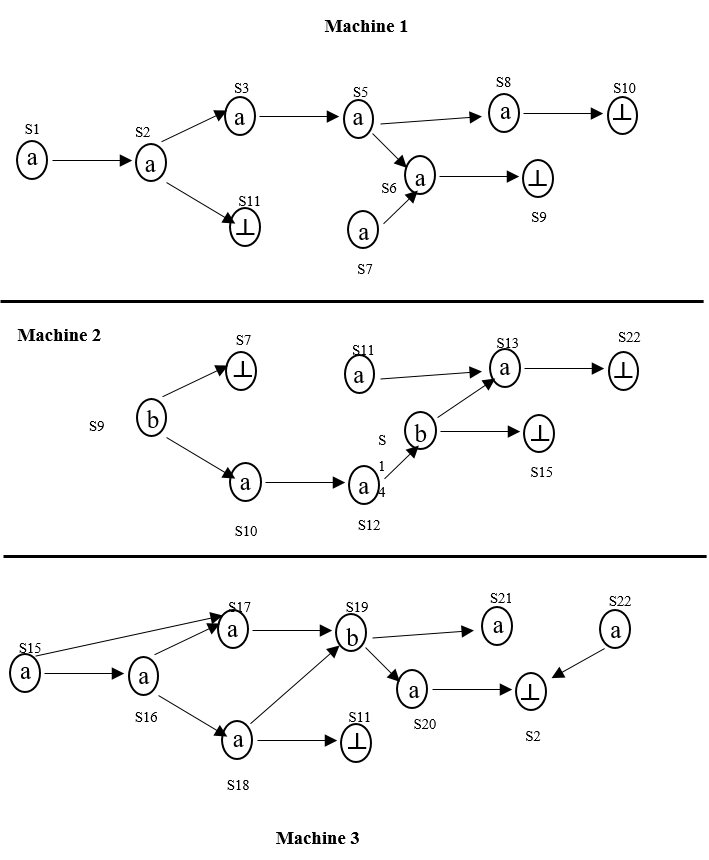
\includegraphics[height=4in]{img/skd2.png}	
	\captionof{figure}{Structure de kripke distribu\'{e}} \label{skd2}
	\end{center}

 
%%%%%%%%%%%%%%%%%%%%%%%%%%%%%%%%%%%%%%%%%%%%%%%%%%%%%%%%%%%%%%%%%%%%%%%%%%%%%%%%%%%%%%%%%%%%%
%%									section Algorithmes	de Redistribution						%
%%%%%%%%%%%%%%%%%%%%%%%%%%%%%%%%%%%%%%%%%%%%%%%%%%%%%%%%%%%%%%%%%%%%%%%%%%%%%%%%%%%%%%%%%%%%%
\makeatother

%L'algorithme de \mcd{} est formalisé comme suit:

	%\begin{fleqn}

%\end{fleqn}

%%%%%%%%%%%%%%%%%%%%%%%%%%%%%%%%%%%%%%%%%%%%%%%%%%%%%%%%%%%%%%%%%%%%%%%%%%%%%%%%%%%%%%%%%%%%%
%%									sub section Initialisation de $\beta ,\gamma $				%
%%%%%%%%%%%%%%%%%%%%%%%%%%%%%%%%%%%%%%%%%%%%%%%%%%%%%%%%%%%%%%%%%%%%%%%%%%%%%%%%%%%%%%%%%%%%%

\subsection{Calcul des valeurs des parametres $\parametretwo{} \; et\;\parametretree{} $ }
 
{L'initialisation des paramètres s'effectue lors de l'exécution du \mc{}. Tel que nous l'avons souligné, ces paramètres  sont initialisés à partir des états sur lesquels la formule n'est pas vérifiée. Par la suite, les états liés sont marqués par chaque état dont ils dépendent (dans l'algorithme c'est la variable \textbf{f} qui stocke cet ensemble d'états). Enfin, les états liés sont énumérés. Un état est dit lié, lorsque la formule n'est pas vérifiée sur ses successeurs directs ou indirects. Certains prédécesseurs directs ou indirects ne sont pas liés aux successeurs directs ou indirects sur lesquels la formule n'est pas vérifiée car celle-ci n'est pas vérifiée sur ces prédécesseurs. Cela motive la duplication de ces états prédécesseurs. A titre d'exemple, l'exécution de la formule  \textit{$AG(a)$} sur la structure de Kripke de la Figure(\ref{skd2}), l'état \sneuf{} est un prédécesseur indirect de l'état \s{S14}, celui-ci peut être dupliqué sur une autre machine car la vérification de la formule sur cet état est indépendante des autres états. 

Dans ce qui suit nous proposons la démarche d'initialisation des paramètres, le marquage des états liés, l'énumération des états liés et des états à dupliquer. Cette démarche est ajoutée à l'algorithme de model checking définit ci-dessus.
}
	\mysubsection{Initialisation des paramètres $\parametretwo{}$  et $\parametretree{} $ }{
Les paramètres $\parametretwo{}$ et $\parametretree{}$ sont initialisés à zéro au niveau des états qui ne comportent pas la formule à vérifier. Lorsque l'état appartient à la machine, le paramètre $\parametretree{}$ sera initialisé à $1$, cela signifie que cet état peut être dupliqué dans les machines qui le référencent. Par exemple, l'exécution de la formule  \textit{$AG(a)$} sur la structure de Kripke distribuée de la Figure(\ref{skd2}) fait qu'à l'état \sneuf{}, le paramètre $\parametretree{}$ est initialisé à 1 pour marquer la duplication de cet état. On remarque que la duplication de l'état \sneuf{}  sur la \mone{}, permet de réduire le temps de vérification de la formule, car la valeur logique de la formule sur à l'état \sneuf{} est connue, la \mtwo{} n'envoie pas alors de message concernant la valeur logique de la formule sur cet état. Le principe d'initialisation est formalisé sur l'équation (\ref{eqn3}). On obtient alors:

\begin{algorithm}[H]\label{alg1}
\SetAlgoLined
\SetKwIF{If}{ElseIf}{Else}{if}{then}{else if}{else}{endif}
\SetKwInOut{S}{$S$}
\SetKwInOut{e}{$e$}
\SetKwInOut{p}{$p$}
\SetKwInOut{ei}{$e.i$}
\SetKwInOut{lep}{$L(e,p)$}
\SetKwInOut{te}{$(type(e)$}
\SetKwInOut{ci}{$\curenti{}$}
\S{Liste des états}
\e{Un état}
\p{Une propriété}
\ei{Liste des itérations d'un état}
\lep{Liste des propriétés d'un états}
\te{Type d'un état: Border pour un état externe}
\ci{Itération courant}
\Begin{	
\ForEach{$e$ in $S$}{\label{line11}
	\If{$(\ L(e,p)=false)\  and\ (e.i=null)\ )$}{\label{line12}
			$e.\parametretwo{}=0$ \;\label{line13}
			$e.\parametretree{}=(type(e)\ne \border{})? \ 0 \ :\ 1 $\; \label{line14}
			$e.i=\{\curenti{} \}$\;\label{line15}
   }
} 
}
 \caption{Initialize Parameters}
\end{algorithm}
Les instructions décrivant l'algorithme(\ref{alg1}) sont expliquées comme suit:
\begin{description}
	\item[ligne \ref{line11} :] Parcourir l'espace d'états d'une \mi{}.
	\item[ligne \ref{line12} :] Vérifier si la formule n'est pas vérifiée sur un état et si une itération précédente n'existe pas (c'est-à-dire si $ e.i\ne null$ alors une itération l'avait déjà initialisée, mais il est à $ null$ . 
	
	Lorsque les conditions de la ligne \ref{line12} sont vérifiées alors les instructions des lignes suivantes sont exécutées:
	\item[ligne \ref{line13} :] Le paramètre $\parametretwo{}$ est initialisé à $0$(zéro).
	\item[ligne \ref{line14} :] Le paramètre $\parametretree{}$ est initialisé à $0$(zéro) lorsque l'état est un \textsl{\border{}} ( c'est-à-dire lorsqu'il appartient à une autre machine ) , sinon à $1$. Par exemple, l'exécution de la formule  \textit{$AG(a)$} sur la structure de Kripke distribuée de la Figure(\ref{skd2}). A l'état \sneuf{} : sur \mone{}  le paramètre $\parametretree{}$ est initialisé à $0$, car cet état n'appartient pas à la machine;  Par contre sur la \mtwo{} le paramètre $\parametretree{}$ est initialisé à $1$, car l'état appartient à cette machine.
	\item[ligne \ref{line15} :] L'itération courante est sauvegardée sur l'état pour éviter de reprendre l'initialisation de cet état lors d'une prochaine itération car s'il n'est pas ajouté, les états respectant les conditions de la ligne \ref{line12} sont initialisés; sans cette initialisation, cet état vérifiera les conditions de la ligne \ref{line12}. 
\end{description}
\begin{Exemple}\label{ea1}
	Après la vérification de la formule \textit{$AG(a)$} sur la structure de Kripke de la Figure (\ref{skd2}), les résultats d'initialisation sont:
\begin{description}
	\item[Itération 1]				
Dans la première itération, le paramètre $\parametretree{}$ est initialisé à $1$ sur tous les états sur lesquels la formule n'est pas vérifiée. L'attribution de la valeur 1 est expliquée au niveau de la ligne \ref{line14} de l'algorithme \ref{alg1}. Par contre le paramètre $\parametretwo{}$ est sans contrainte, alors il est à $0$. Le numéro  d'itération est enregistré sur ces états. La sauvegarde de l'itération courante est expliquée à la ligne \ref{line15} de l'algorithme \ref{alg1}.
Dans le Tableau (\ref{tii1}), on retrouve les états initialisés par les machines.   
\begin{tableth}
	\centering
	\begin{tabular}{|*{6}{c|}}
		\hline
		Id	& $\parametretwo{}$	&$\parametretree{}$&	I&	M&	T\\
		\hline
		S9	&0	&1	&1	&M2	&I\\
		\hline
		S14	&0	&1	&1	&M2	&I\\
		\hline
		S19	&0	&1	&1	&M3	&I\\
		\hline
	\end{tabular}
	\caption{Étape d'initialisation itération 1}\label{tii1}
\end{tableth}	

	\item[Itération 2]				
Après la première itération, les états sur lesquels la formule n'est pas vérifiée, et qui ont des prédécesseurs appartenant à d'autres machines sont notifiées pour prendre en compte la valeur logique de ces états. Une notification déclenche une itération. Elle permet de vérifier la formule sur l'espace d'état de la machine notifiée. Pendant l'itération, l'algorithme du model checker détecte sur certains états que la formule n'est pas vérifiée. Ces états sont liés aux états sur lesquels la notification est faite.
Une seconde itération est déclenchée sur la \mone{}, car l'état \s{S6} dispose d'un successeur sur la \mtwo{} (l'état \s{S9}). La formule n'est pas vérifiée sur cet état(détecté à Itération $1$), d'où la notification envoyée par la \mtwo{} à la \mone{}. Dans la \mone{} les paramètres $(\parametretwo{}, \parametretree{})$ de l'état \s{S9} sont initialisés à zéro. Le paramètre $\parametretree{}$ est initialisé à $0$  parce qu'il n'appartient pas à la \mtwo{}. Ainsi le Tableau (\ref{tii2}) décrit les différents états initialisés dans les machines notifiées.
      
\begin{tableth}
	\centering
	\begin{tabular}{|*{6}{c|}}
		\hline
		Id	& $\parametretwo{}$	&$\parametretree{}$&	I&	M&	T\\
		\hline
		S9&	0&	0&	2&	M1&	E\\
		\hline
		S15&0&	0&	2&	M2&	E\\
		\hline
		S10&0&	0&	2&	M1&	E\\
		\hline
	\end{tabular}
	\caption{Étape d'initialisation itération 2}\label{tii2}
\end{tableth}
	\item[Itération 3]
Après l'itération précédente, des états liés peuvent posséder des prédécesseurs sur d'autres machines. Ces dernières machines  sont notifiées. Par exemple, l'état \s{S2} est lié à l'état \s{S9}, \s{S2} possède des prédécesseurs sur la \mtwo{} et sur la \mtree{}. La notification pour cet état entraine une vérification de la formule sur chaque machine notifiée. Ainsi les paramètres$(\parametretwo{}, \parametretree{})$ de cet état sont initialisées à $0$ d'après l'algorithme d'initialisation. Le paramètre $\parametretree{}$ est initialisé à $0$  parce qu'il n'appartient pas à la machine. Le Tableau (\ref{tii3}) décrit les différents états initialisés sur  chacune des machines.    		 
\begin{tableth}
	\centering
	\begin{tabular}{|*{6}{c|}}
		\hline
		Id	& $\parametretwo{}$	&$\parametretree{}$&	I&	M&	T\\
		\hline
		S7&	0&	0&	3&	M2&	E\\
		\hline
		S2&	0&	0&	3&	M3&	E\\
		\hline
	\end{tabular}
	\caption{Étape d'initialisation itération 3}\label{tii3}
\end{tableth}
	\item[Itération 4] Après l'itération précédente, des états liés peuvent posséder des prédécesseurs sur d'autres machines. Ces dernières sont notifiées. Par exemple l'état \s{S22} est lié à l'état \s{S2}. Il possède un prédécesseur sur la \mtwo{}. La notification pour cet état, déclenche une vérification de la formule sur la \mtwo{}. Ainsi les paramètres$(\parametretwo{}, \parametretree{})$ de cet état sont initialisés à $0$, d'après l'algorithme d'initialisation. Le paramètre $\parametretree{}$ est initialisé à $0$  parce qu'il n'appartient pas à cette machine. Le Tableau (\ref{tii4}) décrit les différents états initialisés sur  chacune des machines. 			  
\begin{tableth}
	\centering
	\begin{tabular}{|*{6}{c|}}
		\hline
		Id	& $\parametretwo{}$	&$\parametretree{}$&	I&	M&	T\\
		\hline
		S22&	0&	0&	4&	M2&	E\\
		\hline
	\end{tabular}
	\caption{Étape d'initialisation itération 4}\label{tii4}
\end{tableth}
	\item[Itération 5] Après l'itération précédente, des états liés peuvent posséder des prédécesseurs sur d'autres machines. Les machines sont notifiées. Par exemple l'état \s{S11} est lié à l'état \s{S2}, des prédécesseurs sont  sur la \mone{} et sur la \mtree{}. La notification pour cet état, déclenche une vérification de la formule sur chaque cette machine. Les paramètres $(\parametretwo{}, \parametretree{})$ de cet état sont initialisés à $0$, d'après l'algorithme d'initialisation. Le paramètre $\parametretree{}$ est initialisé à $0$  parce qu'il n'appartient pas à cette machine. Le Tableau (\ref{tii5}) décrit les différents états initialisés sur chacune des machines.
\begin{tableth}
	\centering
	\begin{tabular}{|*{6}{c|}}
		\hline
		Id	& $\parametretwo{}$	&$\parametretree{}$&	I&	M&	T\\
		\hline
		S11&	0&	0&	5&	M1&	E\\
		\hline
		S11&	0&	0&	5&	M3&	E\\
		\hline
	\end{tabular}
	\caption{Étape d'initialisation itération 5}\label{tii5}
\end{tableth}	
\end{description}	
\end{Exemple}


}
\mysubsection{Marquage des états liés}{
Pendant l'exécution de l'algorithme de vérification, la valeur logique de la formule sur certains états peut dépendre des successeurs directs ou indirects, ces états sont alors liés. La formule peut être vérifiée sur les successeurs, ils peuvent appartenir à d'autres machines. Lorsque la formule n'est pas vérifiée sur un état successeur, les états liés sont alors marqués par cet état. Le principe de marquage est implémenté sur les deux algorithmes de base du model checker. Ils sont définis comme suit : 
\begin{description}
\item[Premier algorithme :] Il est défini par l'équation (\ref{eqn15}), il est utilisé lorsque la vérification concerne tous les successeurs. Ainsi Lorsque la formule n'est pas vérifiée au niveau d'un successeur, deux cas se présentent : 
	\begin{itemize}
		\item La propriété est vérifiée sur l'état, l'état est alors lié à un successeur. Les successeurs sur lesquels la formule n'est pas vérifiée sont marqués sur l'état.
		\item Lorsque la propriété n'est pas vérifiée sur un état, celui-ci peut être dupliqué soit sur la machine réalisant le traitement soit sur des machines distantes. Les états successeurs sur lesquels la formule n'est pas vérifiée sont enregistrés dans l'ensemble \s{limit}, cela signifie que cet état est indépendant de ses successeurs et peut donc être dupliqué sur des machines distantes. Sur l'exemple (\ref{ea1}) de l'Algorithme(\ref{alg1}), la valeur logique de la formule à l'état \s{S9} est indépendante des états \s{S14} et \s{S7}. L'état \s{S9} peut alors être dupliqué sur les machines qui possèdent ses prédécesseurs.
	\end{itemize}  
   
\item[Deuxième algorithme :] Il est défini par l'équation(\ref{eqn16}). Il se différencie du premier algorithme par la vérification de la formule sur les successeurs. Il vérifie l'existence de la propriété sur un successeur. 
\end{description}
En plus des conditions des algorithmes, l'existence de l'itération courante est vérifiée. Cette condition permet de marquer les états de cette itération. Ce principe est formalisé comme suit:\\
\begin{algorithm}[H]\label{alg2}
\SetAlgoLined
\SetKwIF{If}{ElseIf}{Else}{if}{then}{else if}{else}{endif}
$AXf \longleftarrow \emptyset$\; \label{line21}
\ForEach{$e$ in $S$}{\label{line22}
	\uIf{$\left( (\forall e' \; in\; succ(e) \subseteq \left(T^+(f)\cup U^+(f)\right))and(e \in \{T^+(f)\cup U^+(f)\}  )\right)$}{\label{line23}
		$AXf\longleftarrow AXf\cup \left\{e\right\}$\;\label{line24} 
	}
	\Else{\label{line25}
		\uIf{$\left( e\ \;\;in\;\; T \right)$}{\label{line26}
			\ForEach{$e'$ in $succ(e)$}{\label{line27}
				\If{$\left( \curenti{}\;\; in \;\; e'.i \right)$}{\label{line28}
					$e.f\longleftarrow e.f\cup e'.f$\;\label{line29}
					$e.i\longleftarrow e.i\cup \{  \curenti{}\}$\;\label{line210}			
				}			
	   		}\label{endfor27}
   		}\label{line2111}
   		\Else{\label{line211}
   			\ForEach{$e'$ in $succ(e)$}{\label{line212}
				\If{$\left( \curenti{}\;\;in \;\; e'.i \right)$}{\label{line213}
					$e.limit\longleftarrow e.limit\cup e'.f$\;\label{line214}
					$e.fn \longleftarrow e.fn\cup \left\{  \curenti{} \right\}$\; \label{line215}				
				}			
	   		}   		
   		}
	}	
} 
 \caption{Mark linked states formula AX}
\end{algorithm}

Les instructions décrivant l'Algorithme(\ref{alg2}) sont expliquées comme suit:
\begin{description}
	\item[ligne \ref{line21} :] L'ensemble \s{AXf} contient les états sur lesquels la formule est vérifiée ou peut être vérifiée. Cet ensemble est initialisé par l'instruction de cette ligne.
	\item[ligne \ref{line22} :] L'instruction de cette ligne permet de parcourir les états stockés sur la \mi{}
	\item[ligne \ref{line23} :] L'instruction de cette ligne vérifie la formule sur les successeurs, si elle est vérifiée, alors l'instruction de la ligne(\ref{line24}) est exécutée. 
	\item[ligne \ref{line24} :] L'instruction de cette ligne stocke l'état dans l'ensemble \s{AXf}.
	\item[ligne \ref{line25} :] Lorsque la formule n'est pas vérifiée sur l'état ou ses successeurs, les instructions  des lignes suivantes sont alors exécutées. 
	\item[ligne \ref{line26} :] L'instruction de cette ligne vérifie la formule sur l'état. Lorsqu'elle est vérifiée, les instruction des lignes( \ref{line27} à \ref{endfor27}) sont alors exécutées. La ligne \ref{line27} permet de parcourir les successeurs de l'état pour vérifier  l'itération courante grâce à l'instruction de la ligne \ref{line28}. Une fois qu'elle est présente, les instructions suivantes sont exécutées:
	\begin{description}
	\item[ligne \ref{line29} :] L'instruction de cette ligne permet de récupérer les états dont ils dépendent. 
	\item[ligne \ref{line210} :] L'instruction de cette ligne enregistre l'itération courante sur l'état, car un état peut dépendre de plusieurs états de différentes itérations. 
	\end{description}
	\item[ligne \ref{line211} :] Lorsque la formule n'est pas vérifiée sur l'état,ses successeurs sont parcourus grâce à l'instruction de la ligne \ref{line212}. Lors de ce parcours, l'itération courante est vérifiée par l'instruction de la ligne \ref{line213}.\\ Lorsque l'itération courante est présente, les états successeurs sur lesquels la formule n'est pas vérifiée sont enregistrés dans la variable \s{limit} de l'état grâce à l'instruction de la ligne \ref{line214}. La sauvegarde de ces états permet d'éviter le déplacement de cet état, étant donné que sa duplication permet à l'algorithme de connaitre la valeur logique de ces prédécesseurs sans que la machine concernée ne soit notifiée.
	
\end{description}

\begin{algorithm}[H]\label{alg3}
\SetAlgoLined
\SetKwIF{If}{ElseIf}{Else}{if}{then}{else if}{else}{endif}
$EXf \longleftarrow \emptyset$\; \label{line31}
\ForEach{$e$ in $S$}{\label{line32}
	\uIf{$\left( \exists e'  in succ(e) \subseteq \left(T^+(f)\cup U^+(f)\right)\right)$}{\label{line33}
		$EXf\longleftarrow EXf\cup \left\{e\right\}$\; \label{line34}
	}
	\Else{\label{line35}
		\uIf{$\left( e\ \;\;in\;\; T \right)$}{\label{line36}
			\ForEach{$e'$ in $succ(e)$}{\label{line37}
				\If{$\left( \curenti{}\;\;in\;\; e'.i \right)$}{\label{line38}
					$e.f\longleftarrow e.f\cup e'.f$\;\label{line39}
					$e.i\longleftarrow e.i\cup \{  \curenti{}\}$\;\label{line310}				
				}			
	   		}
   		}
   		\Else{\label{line311}
   			\ForEach{$e'$ in $succ(e)$}{\label{line312}
				\If{$\left( \curenti{}\;\; in\;\; e'.i \right)$}{\label{line313}
					$e.limit\longleftarrow e.limit\cup e'.f$\;\label{line314}
					$e.fn \longleftarrow e.fn\cup \left\{  \curenti{} \right\}$\; \label{line315}				
				}			
	   		}   		
   		}
	}\label{line320}	
} 
 \caption{Mark linked states formula EX}
\end{algorithm}

Les instructions décrivant l'Algorithme(\ref{alg3}) sont similaires à celle de l'Algorithme(\ref{alg2}), la différence se trouve au niveau de la vérification de la formule sur les successeurs. Pour l'Algorithme(\ref{alg3}), lorsque la formule est vérifiée ou peut être vérifiée sur un successeur, l'instruction de la ligne \ref{line34} est alors exécutée, sinon les instructions de la ligne \ref{line35} à la ligne \ref{line320} sont exécutées en fonction de la vérification de la formule comme expliqué au niveau de  l'Algorithme(\ref{alg2}).

\begin{Exemple}\label{ea2}
	L'application de l'algorithme de model checker de la formule \textit{$AG(a)$} sur la structure de Kripke de la Figure (\ref{skd2}) donne les états marqués à chaque itération comme suit:
\begin{description}
	\item[Itération 1] Dans la première itération, les états initialisés dans l'exemple(\ref{ea1}) sont utilisés pour déterminer les états liés. Le model checker utilise l'Algorithme(\ref{alg2}) pour vérifier la formule \textit{$AG(a)$}, cet algorithme détecte sur les états(\s{S12},\s{S10}) qu'ils sont liés à l'état \s{S14}, car la formule n'est pas vérifiée sur l'état \s{S14}, par contre la formule est vérifiée sur ces états. La vérification de la formule sur les successeurs directs de l'état \s{S14}, ce dernier est un successeur direct de \s{S12}, ou indirect	s de l'état \s{S14}, ce dernier est un successeur indirect de l'état \s{S10}, cela montre qu'elle n'est pas vérifiée sur chacun de ces états. l'état \s{S14} est marqué dans l'ensemble de dépendance des états liés. L'état \s{S9} est un prédécesseur indirect de l'état \s{S14}, ce dernier est marqué sur l'ensemble \s{limit} de l'état \s{S9} car la formule n'est pas vérifiée sur état \s{S9}. Le Tableau (\ref{tim1}) représente les différents états marqués par chacune des machines pendant cette itération.   
\begin{tableth}
	\centering
	\begin{tabular}{|*{7}{c|}}
		\hline
		Id&		T&			F&	I&	limit&	fn&		M\\
		\hline
		S9&		I&$\emptyset$&$\{	1\}$&	$\{S14\}$&	$\{S14\}$&	M2\\
		\hline
		S10&	I&	$\{S14\}$&$\{	1\}$&$\emptyset$& $\emptyset$ &M2\\
		\hline
		S12&	I&	$\{S14\}$&$\{	1\}$&$\emptyset$&$\emptyset$ &	M2\\
		\hline
		S15&	I&	$\{S19\}$&$\{	1\}$&$\emptyset$&$\emptyset$ &	M3\\
		\hline
		S16&	I&	$\{S19\}$&$\{	1\}$&$\emptyset$&$\emptyset$ &	M3\\
		\hline
		S17&	I&	$\{S19\}$&$\{	1\}$&$\emptyset$&$\emptyset$ &	M3\\
		\hline
		S18&	I&	$\{S19\}$&$\{	1\}$&$\emptyset$&$\emptyset$ &	M3\\		
		\hline
	\end{tabular}
	\caption{Étape de marquage: itération 1}\label{tim1}
\end{tableth}
\\\\	
	\item[Itération 2] Dans cette itération les résultats obtenues dans l'exemple(\ref{ea1}) à l'itération 2 sont utilisés pour déterminer les états liés aux états notifiés(dans l'exemple(\ref{ea1}) une notification provoque l'itération 2 sur la \mone{}, cette notification concerne l'état \s{S9}). Pendant la vérification de la formule, l'algorithme détecte la valeur logique de la formule au niveau des états(\s{S1}, \s{S2}, \s{S3}, \s{S4},\s{S5}, \s{S6}) sur la \mone{}. La valeur logique de cette formule sur ces états dépend de la valeur logique de la formule  sur l'état \s{S9}. Ces états sont des prédécesseurs directs ou indirects de l'état  \s{S9}. Cet état est rajouté à l'ensemble  de dépendance, l'itération courante est ainsi marquée. 
Le Tableau (\ref{tim2}) représente les différents états marqués pendant l'itération 2 de chacune des machines.  
	\begin{tableth}
	\centering
	\begin{tabular}{|*{7}{c|}}
		\hline
		Id&		T&			F&	I&	limit&	fn&		M\\
		\hline
		S1&	I&	$\{S9,S10\}$&	$\{1,2\}$&	$\emptyset$& $\emptyset$&		M1\\ \hline
		S2&	I&	$\{S9,S10\}$&	$\{1,2\}$&	$\emptyset$& $\emptyset$&		M1\\ \hline
		S3&	I&	$\{S9,S10\}$&	$\{1,2\}$&	$\emptyset$& $\emptyset$&		M1\\ \hline
		S5&	I&	$\{S9,S10\}$&	$\{1,2\}$&	$\emptyset$& $\emptyset$&		M1\\ \hline
		S6&	I&	$\{S9\}$	   &	$\{2\}$&	$\emptyset$& $\emptyset$&		M1\\ \hline
		S7&	I&	$\{S9\}$    &	$\{2\}$&	$\emptyset$& $\emptyset$&		M1\\ \hline
		S8&	I&	$\{S10\}$   &	$\{2\}$&	$\emptyset$& $\emptyset$&		M1\\ \hline
		S9&	E&	$\emptyset$&	$\{2\}$&	$\emptyset$& $\emptyset$&		M1\\ \hline
		S10&E&	$\emptyset$&	$\{2\}$&	$\emptyset$& $\emptyset$&		M1\\ \hline
		S14&I&	$\emptyset$&	$\{1\}$&	$\{S15\}$   & $\{S15\}$&			M2\\ \hline
		S15&E&	$\emptyset$&	$\{2\}$&	$\emptyset$& $\emptyset$&		M2\\				
		\hline
	\end{tabular}
	\caption{Étape de marquage: itération 2}\label{tim2}
\end{tableth}
	\item[Itération 3] Dans cette itération les résultats obtenues dans l'exemple(\ref{ea1}) à l'itération 3 sont utilisés pour déterminer les états liés aux états notifiés de l'exemple(\ref{ea1}. Une notification provoque l'itération 3 sur la \mtree{}, cette notification concerne l'état \s{S2}). Pendant la vérification, l'algorithme détecte la valeur logique de l'état(\s{S20}) sur la \mtree{}, elle dépend de l'état \s{S2}. Ce dernier est ajouté à l'ensemble  de dépendance de l'état \s{S20}. Par contre l'état \s{S19} est un prédécesseur indirect de l'état \s{S2}, il est ajouté à l'ensemble \s{limit} de l'état (\s{S19}, car la formule n'est pas vérifiée sur cet état l'à. Toute fois l'itération courante est marquée sur l'état \s{S19}. 
le Tableau (\ref{tim3}) représente les différents états marqués pendant l'itération 3 de chacune des machines. 
	\begin{tableth}
	\centering
	\begin{tabular}{|*{7}{c|}}
		\hline
		Id&		T&			F&	I&	limit&	fn&		M\\
		\hline
		S9&	I&	$\emptyset$&	$\{1\}$&	$\{S7\}$   &	$\{S7\}$&	M2\\ \hline
		S7&	E&	$\emptyset$&	$\{3\}$&	$\emptyset$& $\emptyset$&	M2\\ \hline
		S2&	E&	$\emptyset$&	$\{3\}$&$\emptyset$& $\emptyset$	&	M3\\ \hline
		S19&I&	$\{S19\}$&	$\{1\}$&$\{S2\}$   & $\{S2\}$	&	M3\\ \hline
		S20&I&	$\{S2\}$&	$\{3\}$&$\emptyset$& $\emptyset$&	M3\\ \hline
		S22&I&	$\{S2\}$&	$\{3\}$&$\emptyset$& $\emptyset$&	M3\\ \hline
		
	\end{tabular}
	\caption{Étape de marquage: itération 3}\label{tim3}
\end{tableth}
\\\\\\\\\\
	\item[Itération 4] Dans cette itération les résultats obtenues dans l'exemple(\ref{ea1}) à l'itération 4 sont utilisés pour déterminer les états liés aux états notifiés dans l'exemple(\ref{ea1}. Une notification provoque l'itération 4 sur la \mtwo{}, la notification concerne l'état \s{S22}). Le principe de marquage est similaire à l'itération précédente, le Tableau (\ref{tim4}) représente alors les différents états marqués pendant l'itération 4 de chacune des machines. 
	\begin{tableth}
	\centering
	\begin{tabular}{|*{7}{c|}}
		\hline
		Id&		T&			F&	I&	limit&	fn&		M\\
		\hline
		S11&	I&	$\{S22\}$	&	$\{4\}$			&$\emptyset$	&$\emptyset$	&M2\\ \hline
		S13&	I&	$\{S22\}$	&	$\{4\}$			&$\emptyset$	&$\emptyset$	&M2\\ \hline
		S14&	I&	$\emptyset$	&$\emptyset$	&	$\{S15,S22\}$	&$\{S15,S22\}$	&M2\\ \hline
		S22&	E&	$\emptyset$	&	$\{4\}$			&$\emptyset$	&$\emptyset$	&M2\\ \hline
		
	\end{tabular}
	\caption{Étape de marquage: itération 4}\label{tim4}
\end{tableth}\\

	\item[Itération 5] Dans cette itération les résultats obtenues dans l'exemple(\ref{ea1}) à l'itération 5 sont utilisés pour déterminer les états liés aux états notifiés de l'exemple(\ref{ea1}. Une notification provoque l'itération 5 sur la \mtree{}, la notification concerne l'état \s{11}). Ainsi l'algorithme détecte la valeur logique des états(\s{S15}, \s{S16}, \s{S18}) sur la \mtree{}, elle dépend de l'état \s{S11}. Le principe de marquage est similaire à l'itération 2, on remarque sur ces états l'effet de plusieurs itérations, cela s'explique par le fait que ces états dépendent de plusieurs autres états. Le Tableau (\ref{tim5}) représente les différents états marqués pendant l'itération 5 de chacune des machines.
	\begin{tableth}
	\centering
	\begin{tabular}{|*{7}{c|}}
		\hline
		Id&		T&			F&	I&	limit&	fn&		M\\
		\hline
		S1&		I&$\emptyset$&		$\{1 ,5\}$&	$\{S7\}$&	$\{S7\}$&		M2\\ \hline
		S2&		I&$\emptyset$&		$\{1 ,5\}$&$\emptyset$&$\emptyset$&		M2\\ \hline
		S11&	I&$\emptyset$&		$\{5\}$	&$\emptyset$&$\emptyset$&		M2\\ \hline
		S11& 	E&$\emptyset$&		$\{5\}$&$\emptyset$&$\emptyset$&		M3\\ \hline
		S15&	I&	$\{S19,s11\}$&	$\{1 ,5\}$&$\emptyset$&$\emptyset$&		M3\\ \hline
		S16&	I&	$\{S19,s11\}$&	$\{1 ,5\}$&$\emptyset$&$\emptyset$&		M3\\ \hline
		S18&	I&	$\{S19,s11\}$&	$\{1 ,5\}$&$\emptyset$&$\emptyset$&		M3\\ \hline
	\end{tabular}
	\caption{Étape de marquage: itération 5}\label{tim5}
\end{tableth}\\

\end{description}	
\end{Exemple}\break
} 
\mysubsection{Énumération des états liés}{
Après le marquage des états, on obtient sur les états liés les états dont ils dépendent. Ainsi pour chaque état dépendant, les états qui lui sont liés sont énumérés, cela permet d'attribuer des valeurs aux paramètres $(\parametretwo{}$ et $\parametretree{})$. L'attribution des valeurs peut concerner les états appartenant à la machine locale ou appartenant aux machines distantes. Ces valeurs permettent d'effectuer un redéploiement des états sur la bonne machine. Selon le type de chaque état la technique d'énumération est la suivante:
\begin{description}
\item[\ee{} :] Les états externes(\s{border}) sont des états appartenant aux machines distantes. Lorsque la formule n'est pas vérifiée sur ces états, le nombre d'états liés sont recensés. La valeur calculée est attribuée au paramètre $\parametretwo{}$ de l'état \s{border}. 
Dans l'exemple(\ref{ea2}), la valeur du paramètre $\parametretwo{}$ est égale à $2$ à l'état \s{S22} de la \mtwo{}.
 Ainsi la valeur du paramètre $\parametretree{}$ correspond au nombre d'états pour lesquels l'état \s{border} a été inséré dans leurs ensembles respectifs \s{limit}. Dans le cas des états externes, la duplication de ces états sur une machine donne une structure de Kripke incohérente (la structure obtenue présente des états dupliqués sans aucuns prédécesseurs sur la machine elle même, ce modèle est alors incohérent vis à vis d'une structure de Kripke). Pour obtenir une structure cohérente il est envisageable de déplacer ces états sur d'autres machines tout en laissant les duplicatas sur la machine local. Pour ce faire le paramètre$\parametrefour{}$ est utilisé pour stocker le nombres de ces états à la place du paramètre $\parametretree{}$. La valeur de ce paramètre est calculée similairement  à celle du paramètre $\parametretree{}$.
 L'application de ce principe sur l'exemple(\ref{ea2}) permet d'attribuer la valeur $1$ au paramètre $\parametrefour{}$ à l'état \s{S22} de la \mtwo{}, car cet état est stocké dans l'ensemble \s{limit} de l'état \s{S14}.  
 
\item[\ei{} :]  Les états internes sont des états appartenant à la machine locale. Lorsque ces états disposent des prédécesseurs directs sur d'autres machines distantes, les valeurs des paramètres sont alors calculés. La valeur du paramètre $\parametretwo{}$ correspond aux nombres des successeurs directs et indirects présents entre les état marqués sur l'ensemble de dépendance (la variable \s{\textbf{f}}) de l'état, ce nombre est incrémenté de $1$ car l'état dépend de ces états l'à. Par contre la valeur du paramètre $\parametretree{}$  correspond aux nombre des états internes présents sur l'ensemble de dépendance.
  L'application de ce principe sur l'exemple(\ref{ea2}) permet d'obtenir la valeur $2$ pour le paramètre $\parametretwo{}$ et $0$ pour le paramètre $\parametretwo{}$ à l'état \s{S7} de la \mtwo{}.  
\end{description}

Ces principes sont formalisés comme suit:


\begin{function}
	\setcounter{AlgoLine}{0}
	\caption{getSucess($e:state$): List of State}  
  \SetKwInOut{S}{$ElementSucc$}
  \SetKwInOut{e}{$e$}
  \SetKwInOut{ei}{$e.f$}
  \SetKwInOut{te}{$succ(e)$}
  \S{Liste des états Successeur}
  \e{Un état}
  \ei{Liste que dépendant un état}
  \te{Successeur d'un état: Border pour un état externe}  
 
  	\Begin{
  $ElementSucc	\longleftarrow\emptyset$\;
  \ForEach{$e'\in succ(e)$}{ \label{linef1}
   		\If{$((e'\nexists e.f)and((e'.f\cap e.f)\ne\emptyset)$ }{\label{linef2}
    		 	$ElementSucc\longleftarrow ElementSucc\cup\{e'\}\cup \printlcs{e'}$\;\label{linef3}
    		}
    	}
    	
    \KwRet ElementSucc \;\label{linef4}}
\end{function}

Les instructions  de la fonction \s{getSucc} permettent de récupérer les successeurs directs et indirects entre un état et les états dont-il dépend. La ligne \ref{linef1} permet de parcourir les successeurs directs de l'état afin de vérifier leur dépendance avec lui. Cela est faite à la ligne \ref{linef2}.  Lorsque le successeur est en dépendance avec l'état encours, il est ajouté à l'ensemble des successeurs suivi de l'appel de la fonction \s{getSucc} pour le traitement transitif de ses successeurs. Le résultat retourné par cette fonction  est ajouté  à l'ensemble des successeurs. Ces instructions sont exécutées à la ligne \ref{linef3}. Ainsi, la fonction retournera touts les successeurs de l'état en cours à la fin de son exécution.  
\\

\begin{algorithm}[H]\label{alg4}
\SetAlgoLined
\SetKwIF{If}{ElseIf}{Else}{if}{then}{else if}{else}{endif}

\Begin{
\ForEach{$e$ in $S$}{\label{line42}
	\uIf{$\left((e  \in border(M))and (e\in F) and (e.i==\curenti{})\right)$}{\label{line43}
		\ForEach{$e'$ in $S-\{ e\}$}{\label{line44}
			\uIf{$\left((e  \in e.f)\right)$}{\label{line45}
				$e.\parametretwo{} \longleftarrow e.\parametretwo{} +1$\;\label{line46}
			}
			\uElseIf{$(e \in e'.limit )$}{
				$e.\parametretwo{} \longleftarrow e.\parametretwo{} +1$\;\label{line47}
				$e.\parametrefour{} \longleftarrow e.\parametrefour{} +1$\;\label{line48}				
			}				
		}
	}
	\uElseIf{$\left((e  \in Notifier(M))and (e\in T) and (\curenti{}\in e.i)\right)$}{\label{line49}
		$e.\parametretwo{} \longleftarrow Count(getSucc(e))+1$\;\label{line410}
		\ForEach{$e" \in e.f$}{\label{line411}
					\If{$\left( (Type(e") \ne Border AND  e"!=e\right)$}{\label{line415}
						$e.\parametretree{} \longleftarrow e.\parametretree{} +1$\;
					}
		}\label{line416}
	}	}
} 
 \caption{Count parameters values}
\end{algorithm}

Les instructions décrivant l'Algorithme \ref{alg4} sont expliquées comme suit:

\begin{description}
	\item[ligne \ref{line42} :]  Cette ligne présente une instruction de parcours des états stockés sur la \mi{}.
	\item[ligne \ref{line43} :]  L'instruction de cette ligne vérifie que l'état est \s{externe}, la formule n'est pas vérifiée à cet état, et l'itération courante est marquée sur l'état. La dernière condition permet de calculer les valeurs des paramètres d'un état de l'itération courante vérifiant les deux premières conditions. Lorsque ces conditions sont vérifiées, l'espace d'états est alors parcouru par l'instruction de la ligne \ref{line44}, et calcule les valeurs des paramètres. Pour chaque état est vérifiée:
	
	\begin{itemize}
	\item Si l'état externe est présent dans l'ensemble de dépendance de l'état encours, le paramètre $\parametretwo{}$ de l'état externe est alors incrémenté (ligne \ref{line46}) car cet état est lié à l'état externe.
	\item Sinon, si l'état externe est présent dans l'ensemble \s{limit} de cet état, les paramètres $\parametretwo{}$ et $  \parametrefour{}$ sont alors incrémentés (ligne \ref{line47} et ligne \ref{line48}) car cet état peut être déplacer en laissant un dupliquât sur la machine effectuant le traitement.  
	\end{itemize}
	
	\item[ligne \ref{line49} :] L'instruction de cette ligne vérifie sur l'état l'existence des prédécesseurs directs sur des autres machines distantes, la dépendance des successeurs et la présence de l'itération courante. Lorsque ces conditions sont vérifiées, les successeurs  entre les états liés sont alors calculés, car la valeur du paramètre $\parametretwo{}$ correspond au nombre des successeurs entre l'état et les états dont-il dépend (ligne \ref{line41}). Par contre la valeur du paramètre $\parametretree{}$ correspond au nombre des états dont-il dépend appartenant à la machine locale, les instructions sont de la ligne \ref{line411} jusqu'à la ligne \ref{line416}.
\end{description}

\begin{Exemple}\label{ea3}
	L'application de l'Algorithme(\ref{alg4}) permet de déterminer pour chacun des états de l'exemple(\ref{ea1}), les valeurs des paramètres à travers les résultats de l'exemple(\ref{ea2}). Les valeurs calculées sont: 
	
\begin{description}
	\item[Itération 1] La première itération comptabilise pour chaque état \s{Border} ou \s{Notifer} de l'exemple(\ref{ea1}) à l'itération 1 le nombre des états  qui lui sont liés. Ce nombre est affecté au paramètre  $\parametretwo{}$, par exemple dans l'exemple(\ref{ea2}) aucun état dépend de l'état \s{S9} sur la \mtwo{}. Cependant, il peut-être dupliqué sur la \mone{} car la formule n'est pas vérifiée sur cet état, la valeur du paramètre $\parametretree{}$  est alors égale à $1$. Ainsi, les valeurs des paramètres de l'état \s{S14} ne sont pas calculés car il ne possède pas de prédécesseurs sur chacune des autres machines.
Le Tableau (\ref{tie1}) représente les valeurs des paramètres  des états.	
\begin{tableth}
	\centering
	\begin{tabular}{|*{7}{c|}}
		\hline
		Id&$\parametretwo{}$&	$\parametretree{}$	&$\parametrefour{}$ &	I&	M&	T\\ \hline
		S9&		0&	1	&0&	1&	M2&	Notifier\\ \hline
		S10&	2&	1	&0&	1&	M2&	Notifier\\ \hline
		S15&	3&	1	&0&	1&	M3&	Notifier\\ \hline		
	\end{tabular}
	\caption{Calcul des valeurs des parametres: itération 1}\label{tie1}
\end{tableth}
\item[Itération 2] Dans cette itération les valeurs de l'état \s{S15} sont expliquées car le calcul des paramètres des autres états est similaire à l'itération précédente. Ainsi, dans l'exemple(\ref{ea2}) il n'existe pas d'état dépendant de l'état \s{S15} sur la \mtwo{}, par contre sur l'état \s{S14} il est inséré dans l'ensemble \s{limit}. Ainsi les valeurs des paramètres $\parametretwo{}$ et $\parametrefour{}$  sont égales à $1$ car l'état \s{S14} peut être déplacé sur la \mtwo{}. Cet état est donc dupliqué sur la machine locale. 
Le Tableau (\ref{tie2}) représente les valeurs des paramètres  des états.
\begin{tableth}
	\centering
	\begin{tabular}{|*{7}{c|}}
		\hline
		Id&$\parametretwo{}$&	$\parametretree{}$	&$\parametrefour{}$ &	I&	M&	T\\ \hline
		S2&		6&	0&	&	2&	M1&	Notifier\\ \hline
		S7&		2&	0&	&	2&	M1&	Notifier\\ \hline
		S9&		6&	0&	&	2&	M1&	Border\\ \hline
		S15&	1&	0&	1&	2&	M2&	Border\\ \hline		
	\end{tabular}
	\caption{Calcul des valeurs des parametres: itération 2}\label{tie2}
\end{tableth}
\item[Itération 3] Dans cette itération, la démarche pour l'état \s{S2} est similaire à celle de l'état \s{S15} auquel est associé la démarche de l'itération 1 pour calculer les états liés à cet état. Par contre les autres états sont similaires à l'itération 1. Le Tableau (\ref{tie3}) représente les valeurs des paramètres  des états. 
\begin{tableth}
	\centering
	\begin{tabular}{|*{7}{c|}}
		\hline
		Id&$\parametretwo{}$&	$\parametretree{}$	&$\parametrefour{}$ &	I&	M&	T\\ \hline
		S2&		3&	0&	1&	3&	M3&	Border\\ \hline
		S7&		1&	0&	&	3&	M2&	Border\\ \hline
		S22&	1&	0&	&	3&	M3&	Notifier\\ \hline	
	\end{tabular}
	\caption{Calcul des valeurs des parametres: itération 3}\label{tie3}
\end{tableth}

\item[Itération 4] La démarche de cette itération est similaire à l'itération précédente. Le Tableau (\ref{tie4}) représente les valeurs des paramètres  des états.  
\begin{tableth}
	\centering
	\begin{tabular}{|*{7}{c|}}
		\hline
		Id&$\parametretwo{}$&	$\parametretree{}$	&$\parametrefour{}$ &	I&	M&	T\\ \hline
		S11&	2&	0&	0&	4&	M2&	Notifier\\ \hline
		S2&		3&	0&	1&	4&	M2&	Border\\ \hline
	\end{tabular}
	\caption{Calcul des valeurs des parametres: itération 4}\label{tie4}
\end{tableth}

\item[Itération 5] La démarche de cette itération est similaire à l'itération 3. Le Tableau (\ref{tie5}) représente les valeurs des paramètres  des états.
\begin{tableth}
	\centering
	\begin{tabular}{|*{7}{c|}}
		\hline
		Id&$\parametretwo{}$&	$\parametretree{}$	&$\parametrefour{}$ &	I&	M&	T\\ \hline
		S11&	2&	0&	0&	5&	M1&	Border\\ \hline
		S11&	3&	0&	0&	5&	M3&	Border\\ \hline
		S15&	4&	1&	0&	5&	M3&	Notifier\\ \hline
	\end{tabular}
	\caption{Calcul des valeurs des parametres: itération 5}\label{tie5}
\end{tableth}

\end{description}	
\end{Exemple}
}

\mysubsection{Échange des valeurs des paramètres}{
Après le calcul des valeurs des paramètres, ces valeurs sont envoyées aux machines concernées par l'état. A la réception des valeurs, ces dernières sont stockées sur l'état concerné. Ce prince est formalisé comme suit:
\begin{procedure}[H]
	\setcounter{AlgoLine}{0}	
\caption{SendValueCalculate ($id,\parametretwo{},\parametretree{},\parametrefour{},f$)}

  	\Begin{  
\nl  		\ForEach{$e\in \{Notifier(S)\cup Border(S)\}$}{ \label{linesend1}
\nl   		\If{$(\curenti{} \in e.i)$ }{\label{linesend2}
\nl   			$F=(type(e)==Notifier) ? e : \emptyset$\;\label{linesend3}\\
\nl    		 	\ForEach{$m \in e.site $}{\label{linesend4}
\nl   				$send(e.id,e.\parametretwo{},e.\parametretree{},F,e.\parametrefour{},i)\;\;  to \;\;m.id )$\;
    			}\label{linesend5}
    		}
    	}  
   }  	

\end{procedure}

L'envoi des valeurs concernent les états appartenant aux machines distantes sur lesquels la formule n'est pas vérifiée, et les états locale la formule n'est pas vérifiée qui possèdent des prédécesseurs directs sur d'autres machines. Le parcours de ces états est fait par l'instruction de la ligne \ref{linesend1} de la procédure d'envoi. L'envoi des valeurs concerne les états de l'itération courante, car les valeurs sont échangées après chaque itération. La vérification de la présence de l'itération courante est effectuée à la ligne \ref{linesend2}. Lorsqu'elle est pressente, les valeurs calculées sont envoyées à toutes les machines concernées par cet état. Cela est fait de la ligne \ref{linesend3} jusqu'à la ligne \ref{linesend5}.

\begin{Exemple}\label{ea4}
	Le processus d'envoi des valeurs obtenues dans l'exemple(\ref{ea3}), celui-ci montre que les valeurs de certains états ne sont pas envoyées car ces états ne disposent pas de prédécesseurs directs sur des machines distantes.  Les valeurs envoyées pour chaque état sont décrites comme suit:
	\begin{description}
	\item[Itération 1]
		\begin{itemize}
		\item La \mtwo{} envoie les informations: $id =s9$; $\parametretwo{}=0$; $\parametretree{}=1$; $\parametrefour{}=0$; $f =\{S9\}$; $i=2$ (le paramètre i désigne l'identité de la machine) à la \mone{}.
		\item La \mtwo{} envoie les informations: $id =s10$; $\parametretwo{}=2$; $\parametretree{}=1$; $\parametrefour{}=1$;\\$f =\{S10\}$; $i=2$  à la \mone{}.
		\item La \mtree{} envoie les informations: $id =s15$; $\parametretwo{}=3$; $\parametretree{}=0$; $\parametrefour{}=1$;\\$f =\{s19\}$; $i=3$	 à la \mtwo{}.
		\end{itemize}
	\item[Itération 2]
		\begin{itemize}
			\item La \mone{} envoie les informations: $id =s9$; $\parametretwo{} =6$; $\parametretree{} =0$; $\parametrefour{}=0$;\\$f =\emptyset$, $i=1$ à la \mtwo{}.
			\item  La \mone{} envoie les informations: $id =s10$; $\parametretwo{}=5$; $\parametretree{}=0$; $\parametrefour{}=0$;\\$f =\emptyset$; $i=1$ à la \mtwo{}.
			\item  La \mone{} envoie les informations: $id =s7$ ;$\parametretwo{}=2$; $\parametretree{}=0$; $\parametrefour{}=0$;\\$f =\{s9\}$; $i=1$ à la \mtwo{}.
			\item  La \mone{} envoie les informations: $id =s2$; $\parametretwo{}=5$; $\parametretree{}=0$; $\parametrefour{}=0$;\\$f =\{s9,s10\}$; $i=1$ à la \mtree{}.
			\item  La \mtwo{} envoie les informations: $id =s15$; $\parametretwo{}=1$; $\parametretree{}=0$; $\parametrefour{}=1$;\\$f =\emptyset$; $i=2$ à la \mtree{}.
			\end{itemize}	
\item[Itération 3]
		\begin{itemize}
			\item  La \mtwo{} envoie les informations: $id =s7$; $\parametretwo{}=1$; $\parametretree{}=0$; $\parametrefour{}=1$;\\$f =\emptyset$; $i=1$ à la \mone{}.
			\item  La \mtree{} envoie les informations: $id =s2$; $\parametretwo{}=3$; $\parametretree{}=0$; $\parametrefour{}=1$;\\$f =\emptyset$; $i=3$ à la \mone{}.
			\item  La \mtree{} envoie les informations: $id =s22$; $\parametretwo{}=1$; $\parametretree{}=0$; $\parametrefour{}=0$;\\$f =\{s2\}$; $i=3$ à la \mtwo{}.
			\end{itemize}
		\item[Itération 4]
		\begin{itemize}
			\item  La \mtwo{} envoie les informations: $id =s11$; $\parametretwo{}=2$; $\parametretree{}=0$; $\parametrefour{}=0$;\\$f=\{s22\}$; $i=2$ à la \mone{}.
			\item  La \mtwo{} envoie les informations: $id =s11$; $\parametretwo{}=2$; $\parametretree{}=0$; $\parametrefour{}=0$;\\$f=\{s22\}$; $i=2$ à la \mtree{}.
			\item  La \mtwo{} envoie les informations: $id =s22$; $\parametretwo{}$=2; $\parametretree{}=0$; $\parametrefour{}=0$;\\$f=\emptyset$; $i=2$ à la \mtwo{}.
			\end{itemize}
			\item[Itération 5]
		\begin{itemize}
		\item  La \mone{} envoie les informations: $id =s2$; $\parametretwo{}=5$; $\parametretree{}=0$; $\parametrefour{}=0$;\\$f=\{s9,s10,s11\}$; i=1 à la \mtree{}.
			\item  La \mone{} envoie les informations: $id =s11$; $\parametretwo{}=2$; $\parametretree{}=0$; $\parametrefour{}=0$;\\$f=\emptyset$; $i=1$ à la \mtwo{}.
			\item  La \mtree{} envoie les informations: $id =s11$; $\parametretwo{}=3$; $\parametretree{}=0$; $\parametrefour{}$=0;\\$f =\{s22\}$; $i=2$ à la \mtwo{}.
			\item La \mtree{} envoie les informations: $id =s15$; $\parametretwo{}=3$; $\parametretree{}=0$; $\parametrefour{}=1$;\\$f=\{s19,s11\}$; $i=3$	 à la \mtwo{}.
			\end{itemize}	
	\end{description}

\end{Exemple}

\begin{procedure}[H]
\setcounter{AlgoLine}{0}	
\SetAlgoLined
\LinesNumbered
  \caption{Reception de: $(id,\parametretwo{},\parametretree{},\parametrefour{},f,i)$ par la machine j}
  	\Begin{
  \nl\ForEach{$e\in \; S$}{ \label{linereceve1}
  \nl 		\If{$(e.id==id )$ }{\label{linereceve2}
  \nl 			$x.site[i].\parametretwo{} \longleftarrow \parametretwo{}$\;\\
  \nl 			$x.site[i].\parametretree{} \longleftarrow \parametretree{}$ \;\\
  \nl 			$x.site[i].\parametrefour{} \longleftarrow \parametrefour{}$\;\\
  \nl 			$x.site[i].f\longleftarrow f$\;
   			}
    		} 	
    	}
\end{procedure}

Les instructions décrivant la procédure de réception des valeurs, permettent de stocker les valeurs reçues sur l'état concerné. lorsque la machine reçoit les valeurs, l'état consterné est recherché (la ligne \ref{linereceve1} présente l'instruction du parcours des états). Une fois l'état trouvé, les valeurs reçues sont stockées sur l'état dans l'ensemble \s{site}, il contient les informations des machines sur cet état, l'indice de cet liste représente la clé de la machine. 

\begin{Exemple}\label{ea4}
	En appliquant le processus de réception les valeurs reçues sont stockées sur l'état concerné. Ainsi, nous remarquerons que les valeurs de certains états sont mises à jours avec les itérations.  Les valeurs reçues pour chacun des états sont les suivantes:
	
	\begin{description}
	\item[Itération 1]
		\begin{itemize}
		\item A la réception des valeurs: $id =s9$; $\parametretwo{}=0$; $\parametretree{}=1$; $\parametrefour{}=0$; $f =\{S9\}$; $i=2$ par la \mone{}. Ces dernières sont stockées à l'indice \s{i} de la variable  \s{site} de l'état \s{S9}.
		
		\item A la réception des valeurs: $id =s10$; $\parametretwo{}=2$; $\parametretree{}=1$; $\parametrefour{}=1$; $f =\{S10\}$; $i=2$ par la \mone{}. Ces dernières sont stockées à l'indice \s{i} de la variable  \s{site} de l'état \s{S10}.
		
		\item A la réception des valeurs: $id =s15$; $\parametretwo{}=3$; $\parametretree{}=0$; $\parametrefour{}=1$; $f =\{s19\}$; $i=3$ par la \mtwo{}. Ces dernières sont stockées à l'indice \s{i} de la variable  \s{site} de l'état \s{S15}.
		\end{itemize}
	\item[Itération 2]
		\begin{itemize}
			\item A la réception des valeurs: $id =s9$; $\parametretwo{} =6$; $\parametretree{} =0$; $\parametrefour{}=0$; $f =\emptyset$, $i=1$ par la \mtwo{}. Ces dernières sont stockées à l'indice \s{i} de la variable  \s{site} de l'état \s{S9}.
			
			\item  A la réception des valeurs: $id =s10$; $\parametretwo{}=5$; $\parametretree{}=0$; $\parametrefour{}=0$; $f =\emptyset$; $i=1$ par la \mtwo{}. Ces dernières sont stockées à l'indice \s{i} de la variable  \s{site} de l'état \s{S10}.
			\item  A la réception des valeurs: $id =s7$; $\parametretwo{}=2$; $\parametretree{}=0$; $\parametrefour{}=0$; $f =\{s9\}$; $i=1$ par la \mtwo{}. Ces dernières sont stockées à l'indice \s{i} de la variable  \s{site} de l'état \s{S7}.
			\item  A la réception des valeurs: $id =s2$; $\parametretwo{}=5$; $\parametretree{}=0$; $\parametrefour{}=0$; $f =\{s9,s10\}$; $i=1$ par la \mtree{}. Ces dernières sont stockées à l'indice \s{i} de la variable  \s{site} de l'état \s{S2}.
			\item  A la réception des valeurs: $id =s15$; $\parametretwo{}=1$; $\parametretree{}=0$; $\parametrefour{}=1$; $f =\emptyset$; $i=2$ par la \mtree{}. Ces dernières sont stockées à l'indice \s{i} de la variable  \s{site} de l'état \s{S15}.
			\end{itemize}	
\item[Itération 3]
		\begin{itemize}
			\item  A la réception des valeurs: $id =s7$; $\parametretwo{}=1$; $\parametretree{}=0$; $\parametrefour{}=1$; $f =\emptyset$; $i=1$ par la \mone{}. Ces dernières sont stockées à l'indice \s{i} de la variable  \s{site} de l'état \s{S7}.
			\item  A la réception des valeurs: $id =s2$; $\parametretwo{}=3$; $\parametretree{}=0$; $\parametrefour{}=1$; $f =\emptyset$; $i=3$ par la \mone{}. Ces dernières sont stockées à l'indice \s{i} de la variable  \s{site} de l'état \s{S2}.
			\item  A la réception des valeurs: $id =s22$; $\parametretwo{}=1$; $\parametretree{}=0$; $\parametrefour{}=0$; $f =\{s2\}$; $i=3$ par la \mtwo{}. Ces dernières sont stockées à l'indice \s{i} de la variable  \s{site} de l'état \s{S22}.
			\end{itemize}
		\item[Itération 4]
		\begin{itemize}
			\item  A la réception des valeurs: $id =s11$; $\parametretwo{}=2$; $\parametretree{}=0$; $\parametrefour{}=0$; $f =\{s22\}$; $i=2$ par la \mone{}. Ces dernières sont stockées à l'indice \s{i} de la variable  \s{site} de l'état \s{S11}.
			\item  A la réception des valeurs: $id =s11$; $\parametretwo{}=2$; $\parametretree{}=0$; $\parametrefour{}=0$; $f =\{s22\}$; $i=2$ par la \mtree{}. Ces dernières sont stockées à l'indice \s{i} de la variable  \s{site} de l'état \s{S11}.
			\item  A la réception des valeurs: $id =s22$; $\parametretwo{}=2$; $\parametretree{}=0$; $\parametrefour{}=0$; $f =\emptyset$; $i=2$ par la \mtwo{}. Ces dernières sont stockées à l'indice \s{i} de la variable  \s{site} de l'état \s{S22}.
			\end{itemize}
			\item[Itération 5]
		\begin{itemize}
		\item  A la réception des valeurs: $id =s2$; $\parametretwo{}=5$; $\parametretree{}=0$; $\parametrefour{}=0$; $f =\{s9,s10,s11\}$; $i=1$ par la \mtree{}. Ces dernières sont stockées à l'indice \s{i} de la variable  \s{site} de l'état \s{S2}.
			\item  A la réception des valeurs: $id =s11$; $\parametretwo{}=2$; $\parametretree{}=0$;$\parametrefour{}=0$; $f =\emptyset$; $i=1$ par la \mtwo{}. Ces dernières sont stockées à l'indice \s{i} de la variable  \s{site} de l'état \s{S11}.
			\item  A la réception des valeurs: $id =s11$; $\parametretwo{}=3$; $\parametretree{}=0$; $\parametrefour{}=0$; $f =\{s22\}$; $i=2$ par la \mtwo{}. Ces dernières sont stockées à l'indice \s{i} de la variable  \s{site} de l'état \s{S11}.
			\item A la réception des valeurs: id =s15;$\parametretwo{}$=3 ;$\parametretree{}$=0 ;$\parametrefour{}=1$; $f =\{s19,s11\}$; $i=3$	 par la \mtwo{}. Ces dernières sont stockées à l'indice \s{i} de la variable  \s{site} de l'état \s{S15}.
			\end{itemize}	
	\end{description}
\end{Exemple}
}
%%%%%%%%%%%%%%%%%%%%%%%%%%%%%%%%%%%%%%%%%%%%%%%%%%%%%%%%%%%%%%%%%%%%%%%%%%%%%%%%%%%%%%%%%%%%%
%%									subsection Algorithmes	de Redistribution						%
%%%%%%%%%%%%%%%%%%%%%%%%%%%%%%%%%%%%%%%%%%%%%%%%%%%%%%%%%%%%%%%%%%%%%%%%%%%%%%%%%%%%%%%%%%%%%
\subsection{Algorithme de Redistribution }
 
Après l'envoi des valeurs calculées, les états \emph{Border et Notifier} présentent les valeurs calculées aux paramètres $\parametretwo{}$ et $\parametretree{}$ par la machine locale et les machines distantes. Ces valeurs permettent d'appliquer une stratégie de redistribution des états. La stratégie adoptée est celle d'un jeux non coopératif. Chaque machines cherche a optimisée le temps de calcul de la vérification d'une formule en se focalisant sur l'information que pressente les valeurs calculées par chaque machine. Ainsi, grâce à ces valeurs, sur une machine est calculé calcule l'ensemble minimal des états à envoyer sur une machine distante ainsi que l'ensemble minimal des états à recevoir par cette machine locale. L'envoi des états nécessite la prise en compte de l'équilibrage de charge.  
Dans ce qui suit nous proposons une stratégie de recherche de ces ensembles minimaux d'états à déplacer, dans un sens ou dans l'autre, suivi d'une technique d'envoi de ces ensembles d'états.

\mysubsection{Recherche de l'ensemble minimal des états à importer}{
Dans cette partie l'algorithme permet de chercher sur les valeurs des paramètres $\parametretwo{}$ et $\parametretree{}$  calculées par les machines distantes le couple minimal. Le nombres des états associés à ce couple doit être inférieur au nombre des états associés au couple calculé par la machine locale. Le déplacement de ces états sur une machine distante permet de diminuer le temps de la vérification car l'algorithme détecte la valeur logique de ces états sans qu'une notification ne soit envoyée. Ainsi, le couple minimal est recherché sur les valeurs envoyées par les machines distantes au niveau des états \bn{}, comparées aux valeurs  calculées par la machine sur cet état.  Le couple minimal est celui qui dispose des plus petites valeurs des paramètres calculées  par la machine local sur ces états. Cette recherche est faite en premier temps sur les états ayant une dépendance mutuelle (c'est-à-dire les états distants dépendant l'un de l'autre) car le regroupement de ces états sur une machine diminue le nombre d'itérations de deux. Ainsi, lorsqu'il n'existe pas une dépendance mutuelle entre les états le couple minimum est recherché sur les valeurs envoyées par les machines distantes au niveau des états \bn{}. La formalisation de ce principe est la suivante: 
\begin{function}

\setcounter{AlgoLine}{0}
\SetKwInOut{MG}{$MG$}
\SetKwInOut{Border}{$Border(F)$}
\SetKwInOut{Notifier}{$Notifier(F)$}
\SetKwInOut{F}{$F$}
\SetKwInOut{ebeta}{$e.\parametretwo{}$}
\SetKwInOut{egama}{$e.\parametretree{}$}
\SetKwInOut{esitebeta}{$e.sites[j].\parametretwo{}$}
\SetKwInOut{esitegama}{$e.sites[j].\parametretree{}$}
\SetKwInOut{e}{$e,e'$}
\SetKwInOut{esite}{$e.site$}
\SetKwInOut{esitej}{$e.site[j]$} 
  \F{} 
\e{}
\ebeta{}
\egama{}
\esite{}
\esitej{}
\esitebeta{}
\esitegama{}
\MG{}
\Border{}
\Notifier{}


\Begin{
	 $MG\longleftarrow null$\;\label{lineI0}\\
\nl	  \ForEach{$e\in \; Border(F)$}{ \label{linerI1}
					\ForEach{$e'\in \; Notifier(F) $}{\label{linerI2}
			\For{$j=1$ \KwTo $size(e'.site)$}{\label{linerI3}
				\If{($(e\in e'.f) and (exist(e.site[j]))and(e.\parametretwo{}>e.site[j].\parametretwo{}) 
					and$\;$ ((e'.\parametretwo{}>e'.site[j].\parametretwo{})or(e'.\parametretwo{}==e'.site[j].\parametretwo{} and e'.\parametretree{}>e'.site[j].\parametretree{})) and$\; $(((MG.\parametretwo{}>e'.site[j].\parametretwo{})or(MG.\parametretwo{}==e'.site[j].\parametretwo{}\; and\; MG.\parametretree{}>e'.site[j].\parametretree{})or \;MG ==null)$) 
					)}{\label{linerI4}
					$MG\longleftarrow e'.site[j]$\;\label{linerI5}
				}
			}
								
		}
	}
	\If{$MG==null$}{\label{linerI6}
		\nl\ForEach{$e\in \; \{Border(F)\cup Notifier(F)\}$}{\label{linerI7}
			\ForEach{$site\in e.site $}{\label{linerI8}
				\If{$((e.\parametretwo{}>site.\parametretwo{} )or (e.\parametretwo{}==site[j].\parametretwo{}\; and\; e.\parametretree{}>site.\parametretree{} )) and(MG ==null or ((MG.\parametretwo{}>site.\parametretwo{} )or \;(MG.\parametretwo{}==site[j].\parametretwo{} \;and\; e.\parametretree{}>site.\parametretree{} )))$}{\label{linerI99}
					$MG\longleftarrow e'.site[j]$\;\label{linerI9}
				}
				
			}	   	
		}\label{linerI10}
	}	 	
	\nl \Return MG\label{linerI11} 
}
	\caption{$Search\_ Min\_ States\_DeplaceOnDistantMachine$():state}
\end{function}


Les instructions décrivant la fonction précédente sont expliquées comme suit:
\begin{description}
	\item[ligne \ref{lineI0} :] L'instruction de cette ligne sert à initialiser la variable stockant les informations du couple minimal.
	\item[ligne \ref{linerI1} :] Parcourir les états \s{\border{}} sur lesquels la formule n'es pas vérifiée. Ainsi, pour chaque état parcouru, les états \s{\notifier} sont parcourus à la ligne \ref{linerI2} pour rechercher le couple minimal parmis les valeurs envoyées par les machines distantes au niveau des états en dépendance mutuelle. Le parcours des valeurs envoyées par les machines distantes est fait à la ligne \ref{linerI3}. Ainsi la vérification du couple minimal est faite  à la ligne \ref{linerI4}. Lorsqu'un couple minimal est trouvé le contenue de la variable \s{MG} est alors remplacé par les informations du nouveau couple (ligne \ref{linerI5}).
	\item[ligne \ref{linerI6} :]  L'instruction de cette ligne vérifie qu'aucun minimum n'a été trouvé lors de la recherche précédente. Lorsque la condition est vérifiée les instructions de la ligne \ref{linerI7} jusqu'à la ligne \ref{linerI10} sont alors exécutées.
	\item[ligne \ref{linerI7} :] L'instruction de cette ligne permet de parcourir les états \s{\bn{}} sur lesquels la formule n'es pas vérifiée.
	\item[ligne \ref{linerI8} :]  Pour chaque état, l'instruction de cette ligne parcoure les valeurs calculées par les machines distantes et recherche le couple minimum. La vérification du minimum est faite à la ligne \ref{linerI99}. Ainsi la vérification de cette condition entraine l'exécution de l'instruction de la ligne \ref{linerI9}, cela permet à remplacer l'ancien couple par le nouveau.
	\item[ligne \ref{linerI11} :] L'instruction écrite sur cette ligne permet de retourner les informations du couple minimal.
\end{description}


\nopagebreak
}

\mysubsection{Recherche de l'ensemble minimal des états à déplacer}{
L'ensemble minimal des états à déplacer d'une machine distante correspond au couple minimum des couples($\parametretwo{}$ et $\parametretree{}$) calculés par la machine locale sur les états(\bn{}). Le couple minimum représente la plus petite valeur obtenue au paramètre $\parametretwo{}$ avec une valeur minimale au paramètre $\parametretree{}$. Les états associés à ce couple entrainent un léger déséquilibre qui pourrait être accepté avec l'écart calculé. La recherche de ce couple ($\parametretwo{}$ et $\parametretree{}$) est formalisée comme suit:


\begin{function}
\setcounter{AlgoLine}{0}

\Begin{
  \nl $MF \longleftarrow null$\;\label{linerD0}\\
  \nl\ForEach{$e\in \; \{Border(S)\cup Notifier(S)\}-\{MG\}$}{ \label{linerD1}
  \nl		\uIf{$(MG==null )$ }{\label{linerD2}
  \nl				\ForEach{$site \in x.site$}{\label{linerD3}
  \nl					\If{$((x.\parametretwo{}<site.\parametretwo{} )or (x.\parametretwo{}==site.\parametretwo{}\; and\; (x.\parametretree{}<site.\parametretree{} )) and(MF ==null \;or\; ((MF.\parametretwo{}>x.\parametretwo{} )\;or (MF.\parametretwo{}==x.\parametretwo{} \; and\; MF.\parametretree{}>x.\parametretree{} )))$}{\label{linerD4}
  \nl						$MF\longleftarrow x$\;\label{linerD5}
  					}	
  				}\label{linerD7}
  			}
\nl  			 \Else{\label{linerD6}
 \nl 			 	$site\longleftarrow findById(MG.id,x.site)$\;\label{linerD7}\\
  \nl			 	\If{$((site \ne null) and((MF==null) or (MF.\parametretwo{}>x.\parametretwo{}) or (MF.\parametretwo{}==x.\parametretwo{} and MF.\parametretree{}>x.\parametretree{})) and ((x.\parametretwo{}<site.\parametretwo{}) or (x.\parametretwo{}==site.\parametretwo{} and x.\parametretree{}<site.\parametretree{})) $}{\label{linerD8}
\nl  			 	$MF\longleftarrow x$\;\label{linerD9}
  			 	}			  			 
 \nl 			 }\label{endD}
   		} 	
   \nl\Return MF\label{linerD10} 	
}
\caption{$Search\_ Min \_ States\_ DeplaceOnLocaleMachine(MG:state): State$}\label{Search1}
\end{function}
Les instructions décrivant la fonction \ref{Search1} sont expliquées comme suit:
\begin{description}
	\item[ligne \ref{linerD0} :] L'instruction de cette ligne sert à initialiser la variable stockant les informations du couple minimum.
	
	\item[ligne \ref{linerD1} :] L'instruction de cette ligne permet de parcourir les états \s{\bn{}} sur lesquels la formule n'es pas vérifiée. L'état dont il est possible d'importer ses successeurs ou prédécesseurs à partir d'une machine distante est exclu du parcours.
	\item[ligne \ref{linerD2} :]  L'instruction de cette ligne vérifie qu'il n'existe pas des états à importer. La vérification de cette condition entraine l'exécution des instructions de la ligne \ref{linerD3} jusqu'à la ligne \ref{linerD7}.
	
	\item[ligne \ref{linerD3} :] L'instruction de cette ligne permet de parcourir les valeurs calculées par les machines distantes, ainsi les comparer avec les valeurs calculées par la machine locale, la comparaison est effectuée à la  ligne \ref{linerD4}. Lorsque les valeurs de la machine locale sont minimales l'instruction de la ligne \ref{linerD5}  est exécutée, elle permet de mettre à jours le couple minimal.
	
	\item[ligne \ref{linerD6} :] Lorsqu'il existe des états à déplacer sur une machine distante, un ensemble des états est alors recherché sur la machine locale pour l'envoyer sur la machine distante. La recherche de ce couple minimal est faite de la ligne \ref{linerD7} jusqu'à la ligne \ref{endD}.
	
	\item[ligne \ref{linerD7} :] L'instruction de cette ligne permet de récupérer sur l'état les valeurs envoyées par la machine distante. Les valeurs sont récupérées lorsque l'identité de la machine existe sur l'ensemble des machines de l'état.
	
	\item[ligne \ref{linerD8} :]  L'instruction de cette ligne vérifie l'existence des valeurs de la machine distante et leurs supérioritées à celle calculées par la machine locale sur cet état. Lorsqu'elles sont inférieurs au minimum  courant, l'instruction de la ligne \ref{linerD9} met à jour le contenu de la variable \s{MF} par ce couple.
	
	\item[ligne \ref{linerD10} :] L'instruction écrite sur cette ligne permet de retourner les informations du couple recherché.
\end{description}
\nopagebreak
}

\mysubsection{Envoi d'une requête}{
Après la recherche de l'ensemble minimal des états à déplacer, ces états sont ensuite envoyés à la machine concernée sous forme de requête. La requête peut contenir des états à insérer sur la machine distante ou une demande de l'ensemble des états à déplacer sur la machine distante. Ainsi, l’envoi de la requête est fonction de l'équilibrage de charge.

\begin{itemize}
 \item  Lorsque le résultat de la différence entre le nombre des états à déplacer et le nombre des états à importer  est inférieur ou égale à l'écart calculé la requête envoyée comporte alors les états migrants de la machine locale et une demande des états de la machine distante.
 \item Sinon, si le nombre des états à déplacer est inférieur ou égale à l'écart calculé la requête comporte les états à insérer sur la machine distante.
 \item Sinon, s'il s'agit des états de la machine distante, la requête concerne ces états afin que la machine distante puisse les envoyer à la machine.
 \end{itemize}  
Ce principe est formalisé comme suit:

\begin{procedure} [H]
	\setcounter{AlgoLine}{0}
  	\Begin{	
  		\nl \uIf{$\mid MG.site.\parametretwo{} -MF.\parametretwo{} \mid \leq \parametrefive{}$}{\label{pline1}
  		\nl	$send(element(MF),MG) to  MG.id$\;\label{pline2}
  		}
  		\nl \uElseIf{$MG.site.\parametretwo{} \leq \parametrefive{}$}{\label{pline3}
  		\nl	$send(null,MG)  to MG.id$\;\label{pline4}
  		}
  		\nl \ElseIf{$MF.\parametretwo{} \leq \parametrefive{}$}{\label{pline5}
  		\nl	$send(element(MF),null)  to  MF.id$\;\label{pline6}
  		}
  	}
\caption{$Send\_ Request(MG:state,MF:state)$}
\end{procedure}
Les instructions décrivant la procédure ($Send\_ Request$) sont expliquées comme suit:
\begin{description}
\item[ligne \ref{pline1} :] L'instruction de cette ligne permet de vérifier qu'il est possible de déplacer des états locaux et des états distants. La vérification de cette condition permet d'exécuter l'instruction de la ligne \ref{pline2}, elle permet d'envoyer les états à déplacer et la référence des états à importer. 
\item[ligne \ref{pline3} :] L'instruction de cette ligne permet de vérifier qu'il est possible de déplacer des états distants. La vérification de cette condition permet d'exécuter l'instruction de la ligne \ref{pline4}, elle permet d'envoyer la référence des états à déplacer à la machine distante. 
\item[ligne \ref{pline1} :] L'instruction de cette ligne permet de vérifier qu'il est possible de déplacer des états locaux. La vérification de cette condition permet d'exécuter l'instruction de la ligne \ref{pline2}, elle permet d'envoyer l'ensemble des états à la machine distante. 
\end{description}

\begin{function}
	\setcounter{AlgoLine}{0}
\Begin { 
 \nl 		$states \leftarrow \emptyset$\;	
\\ \nl 		\uIf{$ type(s) ==border$}{
\nl 			\ForEach {$e' \in S$}{
\nl				\If{$s.f\in e'.f \;$}{
\nl					$states \leftarrow states \cup \{ e'\}$\;	
 			      }
\nl 			\ElseIf{$s.f\in e'.limit$}{
\nl 					$states\leftarrow states \cup \{ e'\}$\;\\	
\nl 					duplicate(e') in this machine\;	
 				}
			}
 		}
\nl 		\ElseIf{$e \; \in notifier(S)$}{
\nl			$states\leftarrow getSucc(s)$\;
			\ForEach {$e' \in e.f$}{
\nl 				\uIf{$type(e) \ne border$}{
\nl 					$states\leftarrow states \cup \{ duplicate(e)\}$\;
 				}
\nl 				\Else{
\nl 					$states\leftarrow states \cup \{ e\}$\;
 				}
 			}
 		} 		  		
}
\caption{$element(s:state)$}
\end{function}


\nopagebreak\nopagebreak\nopagebreak
}
\mysubsection{Réception d'une requête}{
A la réception d'une requête les états à insérer sont insérés et les ensemble des états demandés sont envoyés. Lorsque des états sont insérés à la structure de Kripke d'une machine, les valeurs calculées par la machine distante sont alors mises à jour par celles correspondantes à la machine locale pour le bon fonctionnement du protocole. Après ce processus  l'Algorithme \ref{alg6} est relancé. 
Ce principe est formalisé comme suit:
\SetKwFunction{printlcs}{$Receive\_ Request$}
\begin{algorithm}
 \SetAlgoLined\DontPrintSemicolon
  \SetKwFunction{algo}{\printlcs{states :List of State,MG:State}}\SetKwFunction{proc}{proc}
  \SetKwProg{myalg}{Procedure}{}{}
  \myalg{\algo{}}{ 	
  		\If{$size(states)\ne 0$}{\label{prline1}
  			add(states) in  Sj \;\label{prline2}
  		}
  		\If{$MG\ne null)$}{\label{prline3}
  			$send(element(MG),null)  to MG.id$\;\label{prline4}
  		}
  		algorithm \ref{alg6}()\;\label{prline6}
}{}
\end{algorithm}

Les instructions décrivant la procédure ($Receive\_ Request$) sont expliquées comme suit:
\begin{description}
\item[ligne \ref{pline1} :] L'instruction de cette ligne vérifie que des états ont été  envoyés. La vérification de cette condition permet d'exécuter l'instruction de la ligne \ref{prline2}, elle permet de rajouter les états reçus à la structure de Kripke(ligne \ref{pline2}). 
\item[ligne \ref{pline3} :] L'instruction de cette ligne vérifie qu'une demande concernant un ensemble des états a été envoyé. La vérification de cette condition permet d'envoyer l'ensemble des états concernant la demande (ligne \ref{pline4}). 
\item[ligne \ref{pline5} :] L'instruction sur cette ligne permet de relancer le protocole de redistribution afin de rechercher un ensemble des états à déplacer.   
\end{description}
\nopagebreak
}
\begin{Exemple}\label{ea5}
L'exécution du protocole de redistribution sur les résultats générés dans les exemples précédents permet d'obtenir  les résultats suivants:

\begin{description}
\item[Itération 1 :] Pendant la première itération du protocole sur la \mone{}, l'algorithme détecte que les état \s{S7} et \s{S9} sont mutuellement dépendants. Ainsi, les valeurs envoyées par la \mtwo{} sur l'état \s{S7} sont minimales, les états concernant ces valeurs sont à déplacer de la \mtwo{}. Ainsi les états à déplacer de la \mone{} vers la \mtwo{} sont recherchés, l'algorithme détecte que les états liés à l'état \s{S11} sont minimaux. Les états de cet ensemble sont à envoyer sur la \mtwo{}. Après ces deux processus de recherche, les valeurs sont évaluées afin de ressortir la requête à envoyer. L'évaluation montre qu'il est possible d'importer les prédécesseurs de l'état \s{S7} et les prédécesseurs de  l'état \s{S11}.
L'état \s{s2} ne sera pas envoyé parmi les états à déplacer car la \mtree{} possède des prédécesseurs directs de cet état. Après l'envoi des états à déplacer, la \mone{} possède l'état \s{S9}, quant à l'état \s{S1} il est possédé par la \mtwo{}.


Sur la \mtree{} l'algorithme détecte qu'il est possible de déplacer l'état \s{S22} sur la \mtwo{}.


   Après ces redistributions d'états, le protocole détecte qu'il est impossible de redistribuer les états car il risque d'avoir un déséquilibre de charge sur les machines.
   
\end{description}
\centering
	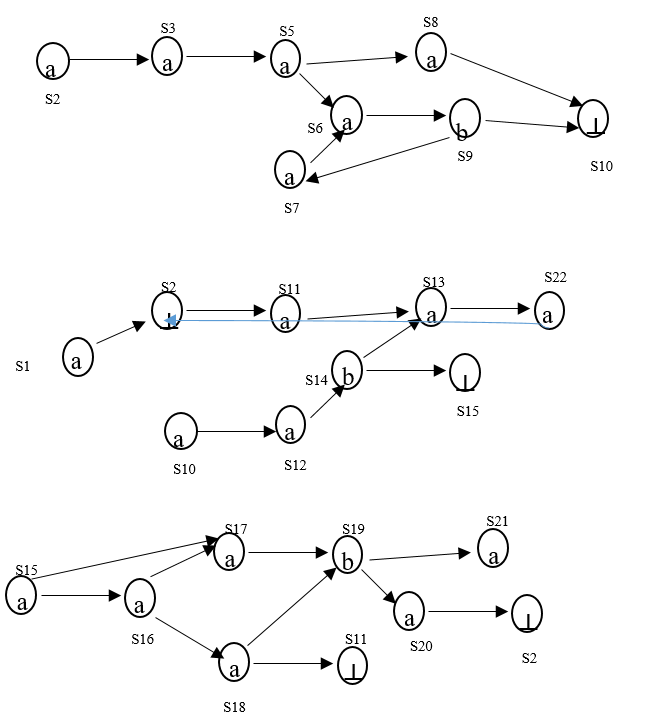
\includegraphics[height=5in]{img/Rskd.png}
	
	\captionof{figure}{Structure de kripke Redistribu\'{e}} 
\end{Exemple}
\section{Étude expérimentale}
Cette section présente les résultats expérimentaux obtenus en appliquant la méthode de redistribution proposée dans ce chapitre.

\subsection{Configuration de la mise en œuvre}
Nous avons développé l’outil qui génère une structure de Kripke distribuée. L’outil dispose d’un éditeur de graphique pour dessiner et modifier les systèmes analysés à partir d'un réseau de Petri (Figure \ref{apppetrinet}).

L’approche proposée a été implémenter avec le langage de programmation JAVA sur IDE IntelliJ, en utilisant le base de donnée orienté graphe Neo4J pour le stockage de l'espace d'états, le Docker pour l'hébergement de ces bases de données. le framework Java Agent Development est aussi utiliser pour faciliter la communication entre les machines.

\section{Conclusion}
Dans ce chapitre, nous avons présenté une nouvelle approche pour la distribution de l’espace d'états basée sur le comportement du système analysé. L’approche proposée vise à améliorer la distribution de l'espace d'états qui sera bénéfique pour le model checking car entraine moins de communication entre les machines. L’approche proposée analyse le comportement d’un système donné, et extrait les informations pertinentes sur ses états. Ensuite, les états sont redistribués suite à leurs pertinences soit migré définitivement soit dupliqués sur d’autres machines, afin de minimiser le nombre de communications entre les machines. La machine récepteur de ces états est choisi suite à la  une stratégie du jeux non coopérative où chaque machine cherche à minimiser le taux de ses communications tout en maintenant un bon équilibrage des états entre les machines à l’aide des seuils prédéfinis pour chaque machine.

L’approche proposée peut être adoptée à tout autre spécification formelle ou modèles d'analyse de données car il pratiquement possible de la formalisée comme un graphe. 